\documentclass[final,c]{beamer}
\mode<presentation>
{
  \usetheme{PaloAlto}
  \usecolortheme{default}
  \setbeamercovered{transparent}
}
\setbeamertemplate{nabigation symbols}{}

\usepackage{luatexja}
\usepackage{luatexja-otf}
\usepackage[match]{luatexja-fontspec}
\usepackage[hiragino-pron,deluxe,expert]{luatexja-preset}

\usepackage{times}
\usepackage[T1]{fontenc}
\usepackage{lmodern}
\usepackage{ascmac}
\usepackage{amssymb,amsmath}
\usepackage{txfonts}
\usepackage{proof}
\usepackage{graphicx}
\usepackage{multimedia}
\usepackage{filecontents}
\usepackage{bxdpx-beamer}
\usepackage{listings}

%\renewcommand{\ttdefault}{lmtl}
\newcommand{\jpy}{{{\ooalign{Y\crcr\hss=\hss}}}}
\newcommand{\lstref}[1]{Listing~\ref{#1}}

\lstset{language=python,%
   basicstyle={\ttfamily\tiny},%
%   lineskip=-0.5zw,%
   commentstyle=\textit,%
   classoffset=1,%
   keywordstyle=\bfseries,%
   breaklines=true,
   frame=lines,%
   framesep=5pt,%
   showstringspaces=false,%
   numbers=left,%
   numbersep=3pt,%
   stepnumber=1,%
   numberstyle={\ttfamily\tiny},%
%   numberstyle={\tiny},%
   numberblanklines=true,
%   morekeywords={def, end, while, if, for, in, else, then, return}%
}%

\title[elementaryCS-1st]{コンピュータサイエンス入門第一\\ \textemdash 3a,4b(CS1)\textemdash}
\date[3rd quarter]{3rd quarter}
\author[Naoyuki Nagatou]{永藤 直行}
\institute[TITECH]{東京工業大学}

\subject{Lecture}

% Delete this, if you do not want the table of contents to pop up at
% the beginning of each subsection:
%\AtBeginSubsection[]
%{
%  \begin{frame}<beamer>{Outline}
%    \tableofcontents[currentsection,currentsubsection]
%  \end{frame}
%}
\AtBeginSection{
  \begin{frame}
\frametitle{Outline}
\scriptsize
\tableofcontents[currentsection]
  \end{frame}
}
\AtBeginPart{\frame{\partpage}}

% If you wish to uncover everything in a step-wise fashion, uncomment
% the following command: 
%\beamerdefaultoverlayspecification{<+->}

\begin{document}
\frame{\titlepage}
%
%%% PROLOGUE
%
\part{Prologue}
\frame{
  \frametitle{Prologue}
  \tableofcontents[part=1]
}
\section{ガイダンス}
%
%%% GOAL
%
\subsection{科目の概要}
\begin{frame}
\frametitle{科目の概要}
  \begin{itemize}
\item 学期: 水曜日 3-4 限
\item 場所: Zoom
\item 担当教員: 永藤 直行 (ナガトウ ナオユキ)
\item 連絡先: nagatou@presystems.xyz
\item 質問時間: メイルか T2Schola の質問用チャットで
\item CS4b クラスのサイト: \href{https://sites.google.com/presystems.xyz/elementarycs/top}{\beamerbutton{https://sites.google.com/presystems.xyz/elementarycs/top}} 
\item 共通サイト: \href{https://wakita.github.io/classes/y21/cs1/course.html}{\beamerbutton{https://wakita.github.io/classes/y21/cs1/course.html}}
\item その他ツールは必要に応じて URL を示します
  \end{itemize}
\end{frame}
%\begin{frame}
%\frametitle{TA の方々}
%  \begin{itemize}
%\item TA の方の自己紹介
%  \end{itemize}
%\end{frame}
%
%%% REFERENCE
%
\subsection{参考図書}
\begin{frame}
\frametitle{参考図書}
  \begin{itemize}
\item 渡辺治 著,コンピュータサイエンス\textendash 計算を通して世界を観る, 丸善出版 (2015)
\item Kenneth H. Rosen 著, Discrete Mathematics and Its Applications 8th ed.(2018)
  \end{itemize}
  \begin{columns}[t]
    \begin{column}{0.45\textwidth}
\centering
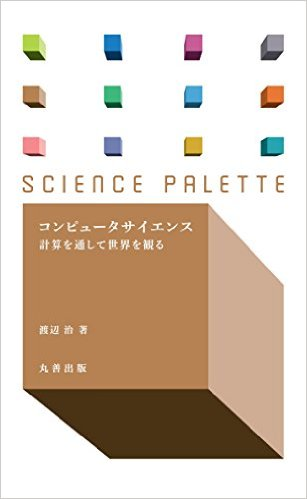
\includegraphics[scale=.25]{./Figure/TextBook.jpg}
    \end{column}
    \begin{column}{0.45\textwidth}
\centering
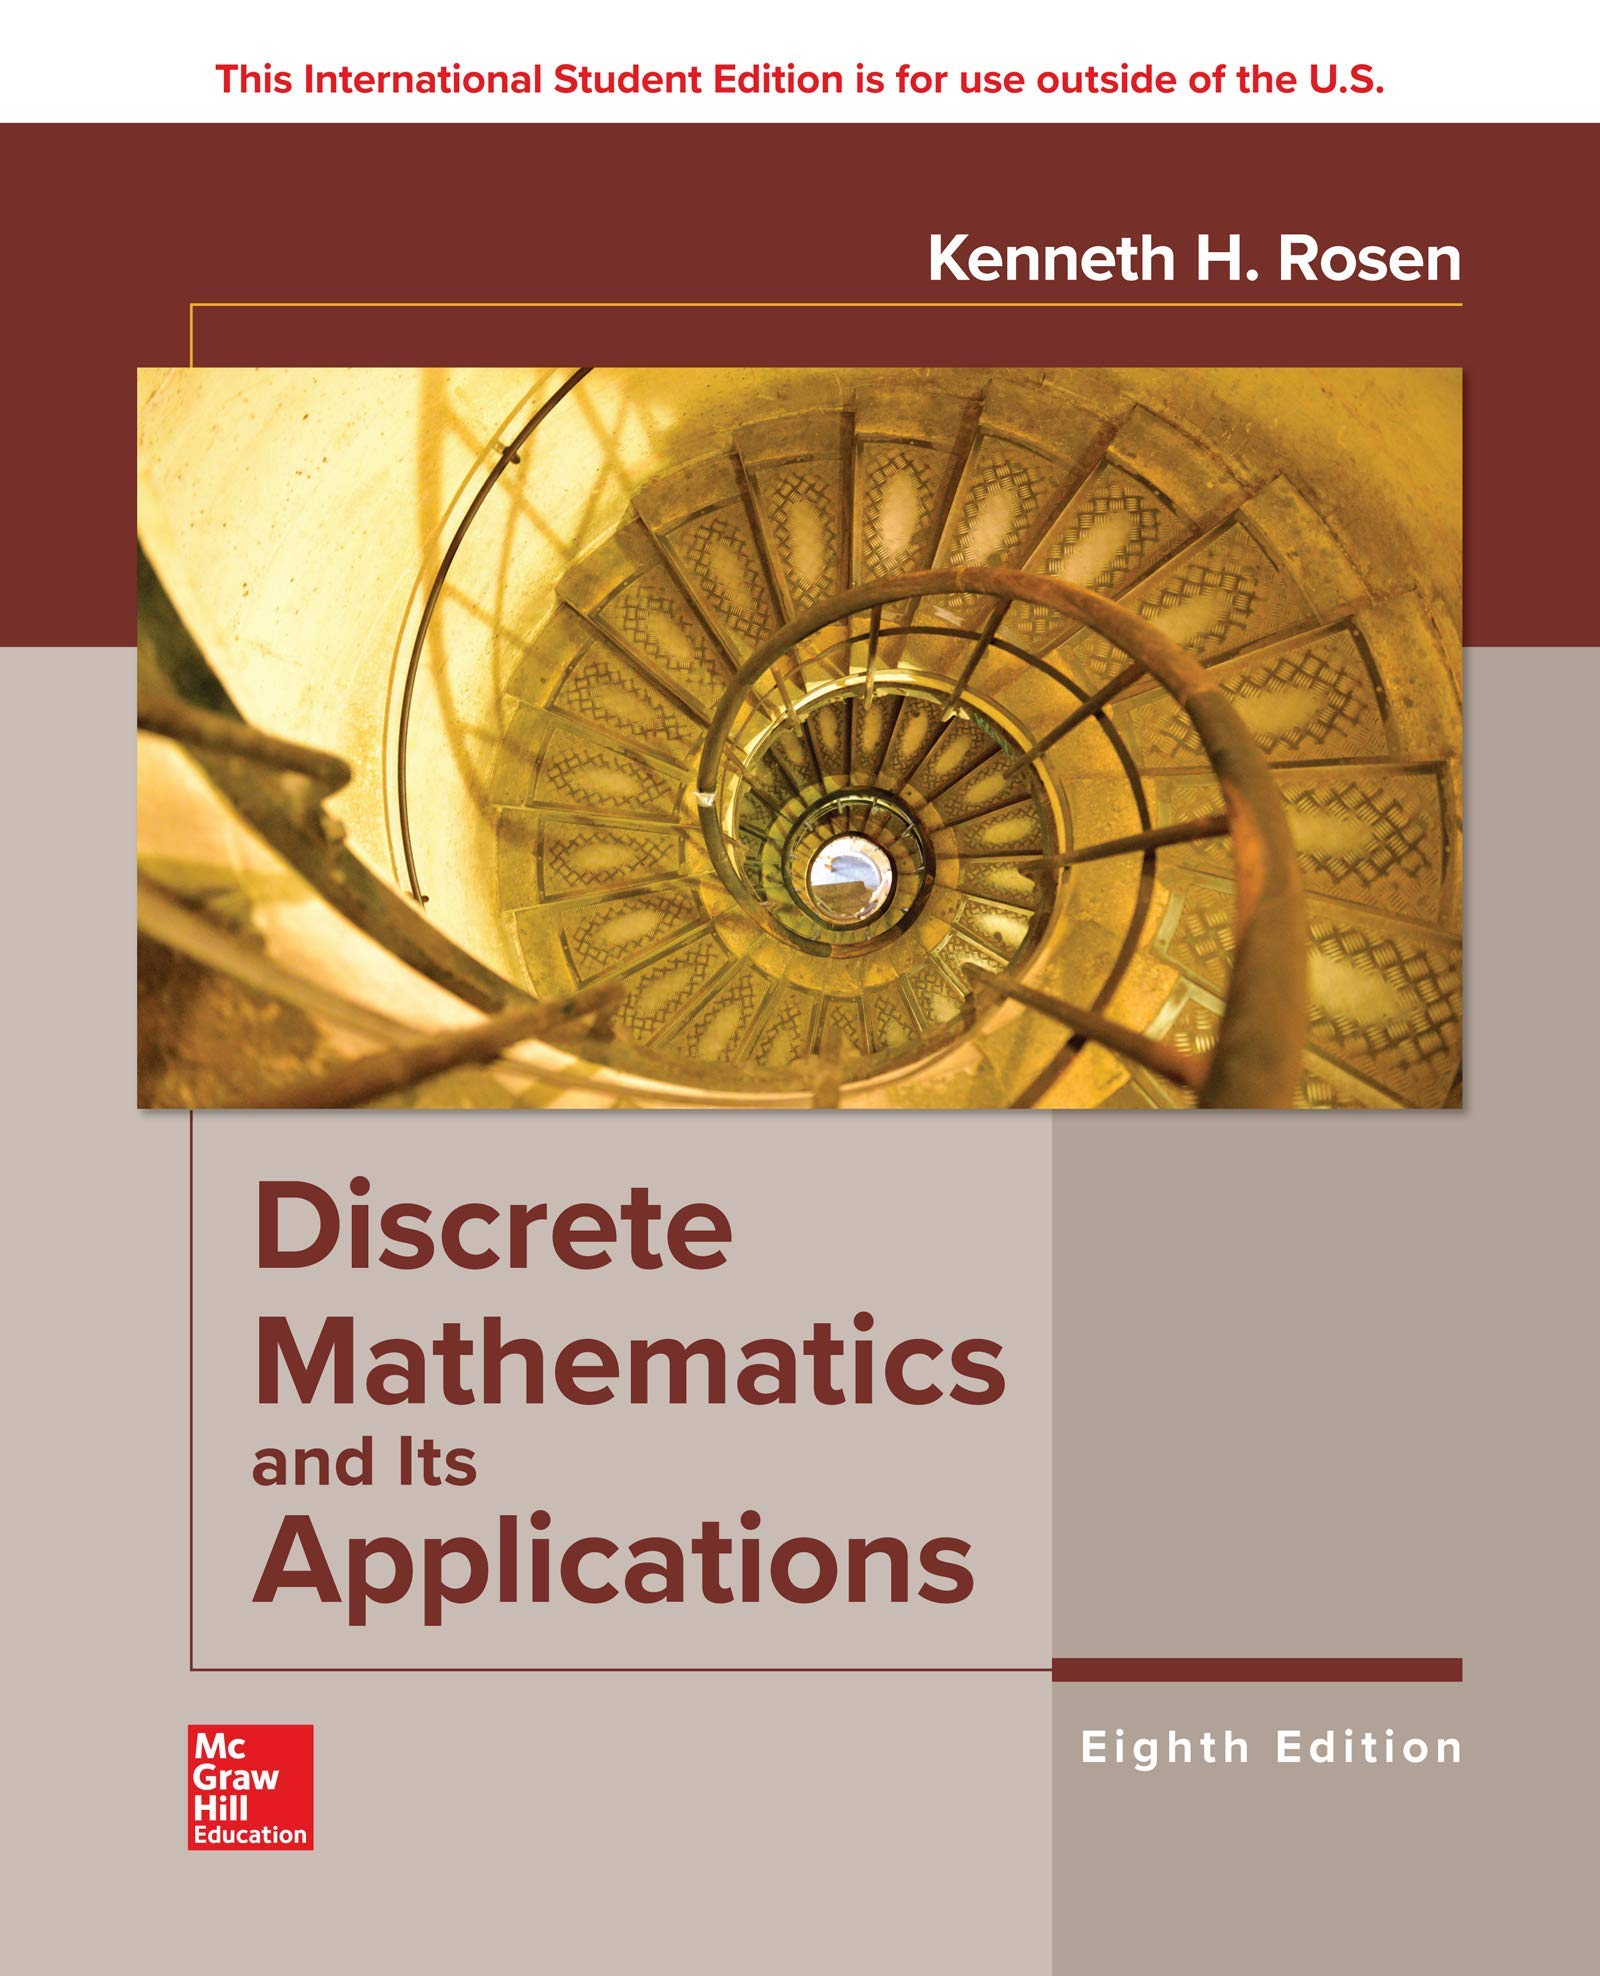
\includegraphics[scale=.07]{./Figure/DMA.jpg}
    \end{column}
  \end{columns}
\end{frame}
%
%%% EVALUATION
%
\subsection{評価基準}
\begin{frame}
\frametitle{評価基準}
  \begin{itemize}
\item 講義は全 7 回,期末試験は行いません
\item 宿題: 3 回 くらい(提出不要)
\item 課題: 4 回 \(25+30+30=85\) 点
\item 特別課題: 1 回 \(15\) 点(提出任意)
\item 宿題・課題提出: 
    \begin{itemize}
\item 講義時間中に課題を出します
\item 提出方法はその都度指定します
    \end{itemize}
\item 宿題と課題提出で出欠確認に変えます
  \end{itemize}
\end{frame}
%
%%% 3rd Quarter Schedule
%
%\subsection{講義スケジュール}
%\begin{frame}
%\frametitle{講義日程}
%  \begin{itemize}
%\item 教室を間違えないように
%\item 進捗によってはまとめと試験は同一日に実施するかも
%  \end{itemize}
%  \begin{center}
%    \begin{tabular}{rll}
%回&題目&場所\\
%\hline
%1&ガイダンス,環境構築,計算の基礎& Zoom\\
%2&プログラミング演習&  Zoom\\
%3&配列,文字列& Zoom\\
%4&プログラミング演習& Zoom\\
%5&暗号入門& Zoom\\
%6&プログラミング演習& Zoom\\
%7&まとめ& Zoom
%%7&試験& 西 2 号館 W631
%    \end{tabular}
%  \end{center}
%\end{frame}

\section{CS 講義概要}
%
%%% GOAL
%
\subsection{講義の目標}
\begin{frame}
\frametitle{講義の目標}
  \begin{itemize}
\item 本講義では,このコンピュータサイエンスの基本をなす考え方を,課題をやることを通して体得する
\item 物理現象をシミュレートしたり
\item 経済活動にともなう帳票類を管理したり
\item 機器を制御したり
\item コンピュータがいろいろな場面で利用されている
  \end{itemize}
\centering
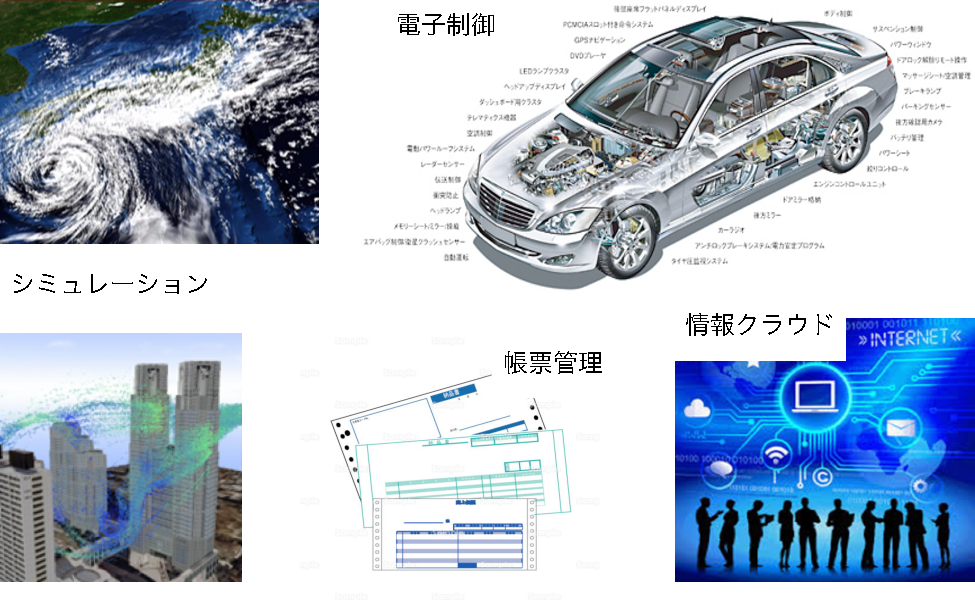
\includegraphics[scale=.35]{./Figure/elementaryCS-1st-FigComputer.pdf}
\end{frame}
\subsection{講義内容}
\begin{frame}
\frametitle{コンピュータに載せるとは?}
  \begin{itemize}
\item なぜコンピュータが利用できるのか
\item どうやってコンピュータに載せるのか
  \end{itemize}
  \begin{block}{コンピュータに載せる}
やりたいことを\emph{計算}をもちいて表現し,コンピュータに処理させること
  \end{block}
  \begin{block}{目標}
    \begin{itemize}
\item CS 第一
      \begin{itemize}
\item 計算で表現するとは何か
\item コンピュータで処理するとは
      \end{itemize}
\item CS 第二 \href{http://www.is.c.titech.ac.jp/~is0000_kashima/CSpublic/3Q.html}{\beamerbutton{第二の講義概要}}
      \begin{itemize}
\item 計算の強力な道具 $\Rightarrow$ 再帰
\item 載せ方の上手下手があること $\Rightarrow$ アルゴリズムやデータ
      \end{itemize}
    \end{itemize}
  \end{block}
\end{frame}
\begin{frame}
\frametitle{講義内容}
  \begin{itemize}
\item 以下の演習を通して実感しながら理解していく
  \end{itemize}
  \begin{block}{演習内容}
    \begin{itemize}
\item 演習課題 1: 四則演算でアニメーション
      \begin{itemize}
\item 計算の基本要素を知る
      \end{itemize}
\item 演習課題 2: 循環小数
      \begin{itemize}
\item 配列とは
      \end{itemize}
\item 演習課題 3: 暗号解読に挑戦
      \begin{itemize}
\item プログラミングとは
\item 計算の組み立て方
      \end{itemize}
    \end{itemize}
  \end{block}
\end{frame}

%
%%% PROGRAMMING ENVIRONMENT
%
%\section{開発環境構築}
\subsection{Python3 環境構築}
\begin{frame}[shrink]
\frametitle{環境構築}
\framesubtitle{Python3}
  \begin{itemize}
\item Python を利用するためには各自の PC 上に環境を構築する必要があります
\item すでに python 開発環境を持っている人は以下の作業は不要です
\item 各状況に合わせて環境を作っていきます
    \begin{itemize}
\item Cloud で利用したい方は\href{https://www.pythonanywhere.com/}{\beamerbutton{https://www.pythonanywhere.com/}}で beginner account を作成(無料でインストール不要です)
\item Windows, Mac OSX, Linux で自分の PC に環境を作りたい方は\href{https://www.python.jp/install/install.html}{\beamerbutton{https://www.python.jp/}}を参照
    \end{itemize}
  \end{itemize}
\end{frame}
\begin{frame}[shrink,containsverbatim]
\frametitle{Pythonanywhere のアカウント開設}
  \begin{itemize}
\item ``Start running Python on line in less than a minute'' をクリック
  \end{itemize}
\includegraphics[width=1\textwidth]{../InformationLiteracy/Figure/IL-figStartAnywhere.jpg}
\end{frame}
\begin{frame}[shrink,containsverbatim]
\frametitle{Pythonanywhere のアカウント作成}
  \begin{itemize}
\item ``Create a Biginner account'' をクリック
\item 無料のアカウントを作成します
  \end{itemize}
\includegraphics[width=1\textwidth]{../InformationLiteracy/Figure/IL-figCreateAnywhereAccount.jpg}
\end{frame}
\begin{frame}[shrink,containsverbatim]
\frametitle{Pythonanywhere のアカウント登録}
  \begin{itemize}
\item ``Username'' を入力(任意)
\item ``Email'' を入力(m ドメイン以外でもかまいません)
\item ``Password'' を入力
\item ``I agree$\ldots$'' にチェック
\item ``Register'' をクリック
  \end{itemize}
\includegraphics[width=1\textwidth]{../InformationLiteracy/Figure/IL-figAnywhereRegister.jpg}
\end{frame}
\begin{frame}[shrink,containsverbatim]
\frametitle{登録後の画面}
  \begin{itemize}
\item 登録アドレスにメイルが届くので確認
\item 以下のような画面が見えれば OK
  \end{itemize}
  \begin{itembox}{登録後の画面}
\includegraphics[width=1\textwidth]{../InformationLiteracy/Figure/IL-figAnywhereDashboard.jpg}
  \end{itembox}
\end{frame}
\begin{frame}[shrink,containsverbatim]
\frametitle{自身の PC 上にインストールひと}
  \begin{itemize}
\item Idle を起動してください
  \end{itemize}
  \begin{columns}[t]
    \begin{column}{0.5\textwidth}
      \begin{itembox}{\footnotesize Mac, Linux のひと}
        \begin{itemize}
\scriptsize
\item ターミナルを起動して idle3 と入力
        \end{itemize}
        \begin{verbatim}
> idle3
        \end{verbatim}
      \end{itembox}
    \end{column}
    \begin{column}{0.5\textwidth}
      \begin{itembox}{\footnotesize Windows のひと}
        \begin{itemize}
\item スタートメニューから IDLE を起動
        \end{itemize}
      \end{itembox}
    \end{column}
  \end{columns}
\end{frame}
\begin{frame}[shrink,containsverbatim]
\frametitle{開発統合環境}
\framesubtitle{IDLE と Pythonanywhere}
  \begin{itemize}
\item Mac, Windows, Linux の人もこれで準備ができました
\item それぞれ以下のような画面が見えるはずです
\item 以後,いずれかの開発統合環境を利用していきます
\item Pythonanywhere や IDLE は編集,実行が統合された環境を提供しています
\item IDLE の使い方は\href{https://docs.python.org/ja/3/library/idle.html?highlight=idle}{\beamerbutton{Python 公式}}を参照
    \begin{itemize}
\item \href{http://www.isc.meiji.ac.jp/~mizutani/python/intro1_python.html}{\beamerbutton{http://www.isc.meiji.ac.jp/~mizutani/python/intro1\_python.html}}も参考になるかも
    \end{itemize}
  \end{itemize}
  \begin{columns}[c]
    \begin{column}{5cm}
\includegraphics[width=1\textwidth]{../InformationLiteracy/Figure/IL-figIDLE.jpg}
    \end{column}
    \begin{column}{5cm}
\includegraphics[width=1\textwidth]{../InformationLiteracy/Figure/IL-figPythonanywhere.jpg}
    \end{column}
  \end{columns}
\end{frame}
\subsection{動作確認}
\begin{frame}[shrink,containsverbatim]
\frametitle{開発環境テスト用コード}
%\vspace{-2zw}
%  \begin{lstlisting}[caption={環境テスト用コード},label=lst:test,numbers=none]
%import matplotlib.pyplot as plt
%print('Hello World')
%plt.plot([1, 2, 3, 4])
%plt.show()
%  \end{lstlisting}
  \begin{itemize}
\item \href{https://sites.google.com/presystems.xyz/elementarycs/top}{\beamerbutton{https://sites.google.com/presystems.xyz/elementarycs/top}} 
からhello.pyをダウンロード
  \end{itemize}
\vspace{-1em}
  \begin{columns}[t]
    \begin{column}{0.5\textwidth}
      \begin{itembox}{\footnotesize IDLE 利用のひと}
        \begin{itemize}
\scriptsize
\item File->Open で hello.py を開く
        \end{itemize}
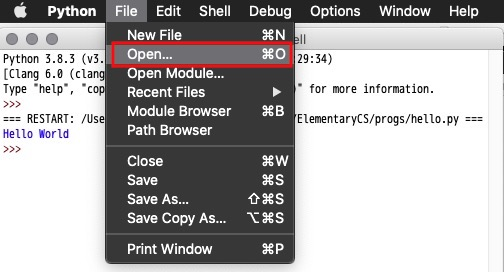
\includegraphics[width=1\textwidth]{./Figure/elementaryCS-figOpenFile.jpg}
      \end{itembox}
    \end{column}
    \begin{column}{0.5\textwidth}
      \begin{itembox}{\footnotesize Pythonanywhere 利用のひと}
\scriptsize
        \begin{itemize}
\item 右上 ``Files'' をクリック
\item ''upload'' をクリックして hello.py をアップロード
\item hello.py をクリックすると中が見れます
        \end{itemize}
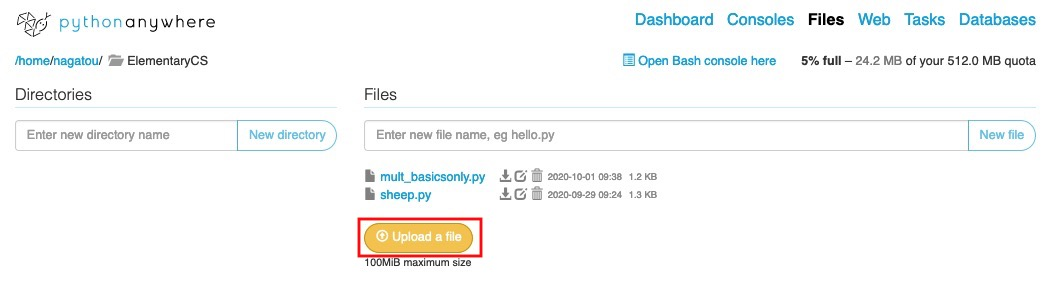
\includegraphics[width=1\textwidth]{./Figure/elementaryCS-figUpload.jpg}
      \end{itembox}
    \end{column}
  \end{columns}
\end{frame}
\begin{frame}[shrink,containsverbatim]
\frametitle{プログラムの実行}
%  \begin{itemize}
%\item \href{https://sites.google.com/a/presystems.xyz/sample/home/information-literacy}{\beamerbutton{https://sites.google.com/a/presystems.xyz/sample/home/information-literacy}}から test.py をダウンロード
%  \end{itemize}
  \begin{columns}[t]
    \begin{column}{0.5\textwidth}
      \begin{itembox}{\footnotesize IDLE 利用のひと}
        \begin{itemize}
\scriptsize
\item Run->Run Module をクリック
\item ``Hello World'' が表示されれば正常
        \end{itemize}
\includegraphics[width=1\textwidth]{../InformationLiteracy/Figure/IL-figTestIDLE.jpg}
      \end{itembox}
    \end{column}
    \begin{column}{0.5\textwidth}
      \begin{itembox}{\footnotesize Pythonanywhere 利用のひと}
\scriptsize
        \begin{itemize}
\item Run this file をクリック
\item 下半分の黒い画面に ``Hello World'' と表示されれば正常
\item 下半分の黒い画面で exit() と入力してください
        \end{itemize}
\includegraphics[width=1\textwidth]{../InformationLiteracy/Figure/IL-figTestCloud.jpg}
      \end{itembox}
    \end{column}
  \end{columns}
\end{frame}

\section{情報の格納}
\subsection{教育用計算機ステムの利用開始}
\begin{frame}[shrink]
\frametitle{教育用システムの利用}
  \begin{itemize}
\item \href{http://www.edu.gsic.titech.ac.jp/}{\beamerbutton{教育用電子計算機システム}}のサイトの``アカウント利用開始''を参照
  \end{itemize}
  \begin{center}
\includegraphics[scale=.3]{../InformationLiteracy/Figure/iMac.jpg}
  \end{center}
\end{frame}
\subsection{ファイル}
\begin{frame}[shrink]
\frametitle{情報の格納}
\framesubtitle{ファイルとディレクトリ (フォルダ)}
  \begin{itemize}
\item さまざまなタイプの情報をビットの列として記録しいてます
    \begin{itemize}
\item 数値,文字,図,表,写真,音声,動画など情報のあらゆるタイプ
    \end{itemize}
\item コンピュータの中では情報をファイルやディレクトリ(フォルダ)と云うもので管理しています
\item ファイル
    \begin{itemize}
\item コンピュータ内の情報はファイルという単位で扱われる
\item e.g. テキストファイル,画像ファイル,音声ファイルなど
    \end{itemize}
\item ディレクトリ
    \begin{itemize}
\item ファイルの入れ物
    \end{itemize}
\item 名前はすきなものをつけられます
    \begin{itemize}
\item でも漢字は使わないほうがいいです
\item アルファベットと記号だけで名前を付けるほうがいいです
    \end{itemize}
  \end{itemize}
\end{frame}
\begin{frame}
\frametitle{ファイルの形式}
  \begin{itemize}
\item さまざまな情報がビット列であらわされ,コンピュータで編集,加工することができます
\item 編集,加工するにはプログラムが必要になります
\item しかし,ビットの列というだけでは何のデータか分かりません
\item ファイルに納められているデータが何のデータであるか約束が必要です
\item それがファイル形式ということになります
\item ファイルの形式は拡張子(suffix)と呼ばれるもので示されていることが多い
    \begin{itemize}
\item .csv, .txt, .c, .obj, .pdf, .doc, .mid などなど
%\item .txt, .c, .obj, .pdf, .doc, \movie[once,externalviewer]{\beamerbutton{.mid}}{./Materials/Gundam.mid}  などなど
    \end{itemize}
\item 形式ごとにプログラムが対応づけられています
  \end{itemize}
\end{frame}
\begin{frame}
\frametitle{ファイルに対する操作}
\scriptsize
  \begin{tabular}{l|l|lp{4cm}}
操作 & コマンド & 実行例 & \\\hline
生成 & touch & touch $name$ & 指定した名前で空のファイルを生成\\
名前変更 & mv & mv $oldfile\ newfile$ & $oldfile$ という名前を $newfile$ という名前に変更\\
複製 & cp & cp $srcfile\ dstfile$ & $srcfile$ を複製して $dstfile$ という名前をつける\\
表示 & less & less $name$ & $name$ の内容を表示\\
消去 & rm & rm $name$ & 指定した名前のファイルを消去
  \end{tabular}
\end{frame}
\subsection{ディレクトリ (フォルダ)}
%\begin{frame}
%\frametitle{ディレクトリ}
%  \begin{itemize}
%\item コンピュータを利用しているとファイルはだんだん増えて必要なファイルを探しだすのが難しくなります
%\item 増えてきたら幾つかのグループに分けて管理すると便利です
%\item ファイルを入れる箱をディレクトリとよんでいます.
%\item 箱に箱を入れることができるようにディレクトリにディレクトリを入れることもできます
%  \end{itemize}
%  \begin{center}
%\includegraphics[scale=.3]{../InformationLiteracy/Figure/IL-figDir.pdf}
%  \end{center}
%\end{frame}
\begin{frame}
\frametitle{ディレクトリの階層}
  \begin{itemize}
\footnotesize
\item ファイルはすべて異なる名前をつけなければなりません
\item ファイルはだんだん増えて違う名前を考えるのは難しくなるかもしれません
\item 複数のユーザが利用しているので知らないうちに同じなまえになっているかもしれません
\item 階層化して管理すると便利です
\item 特定のディレクトリ内の高々数個のファイルならば違う名前を付けるのは容易なはず
  \end{itemize}
  \begin{center}
\includegraphics[scale=.3]{../InformationLiteracy/Figure/IL-figPath.pdf}
  \end{center}
\end{frame}
\begin{frame}
\frametitle{作業ディレクトリあるいは current directory}
  \begin{itemize}
\item ファイルをディレクトリごとに整理できたら,操作は特定のディレクトリのファイルを対象にするとおもいます
\item 作業するときには利用者がその場所まで移動します
    \begin{itemize}
\item 場所とはいってもコンピュータ内でのこと
    \end{itemize}
\item 自分が今いるディレクトリを作業ディレクトリあるいは current directory と呼びます
  \end{itemize}
  \begin{center}
\includegraphics[scale=.3]{../InformationLiteracy/Figure/IL-figPath.pdf}
  \end{center}
\end{frame}
\begin{frame}[containsverbatim]
\frametitle{パス}
  \begin{itemize}
\item コンピュータ内の場所はパス (path) で表します
\item パス (path) は \slash でディレクトリ名を区切った文字列
    \begin{itemize}
\item e.g. \verb|~/literacy| と云ったような文字列
    \end{itemize}
\item ディレクトリにはルートディレクトリとホームディレクトリと呼ぶ特別なディレクトリがあります
\item 絶対パスと相対パス
  \end{itemize}
  \begin{center}
\includegraphics[scale=.3]{../InformationLiteracy/Figure/IL-figPath.pdf}
  \end{center}
\end{frame}
\begin{frame}
\frametitle{ディレクトリに対する操作}
\scriptsize
  \begin{tabular}{l|l|lp{4cm}}
操作 & コマンド & 実行例 & \\\hline
作成 & mkdir & mkdir $name$ & 指定した名前で空のディレクトリを生成\\
一覧 & ls & ls $dir$ & $dir$ の中身一覧を表示\\
格納 & mv & mv $file\ dir$ & $file$ を消去して $dir$ に格納\\
     & cp & cp $file\ dir$ & $file$ を複製して $dir$ に格納\\
名称変更 & mv & mv $olddir\ newdir$ & $olddir$ を $newdir$ に変更\\
消去 & rmdir & rmdir $dir$ & 空の時には $dir$ を消去\\
     & rm    & rm -r $dir$ & 中身ごと $dir$ を消去\\
移動 & cd & cd $dir$ & 作業ディレクトリを移動\\
     & pushd & pushd $dir$ & 作業ディレクトリを移動して現在のディレクトリを保存\\
     & popd & popd $dir$ & 作業ディレクトリを保存したディレクトリに移動\\
表示 & pwd & pwd & 作業ディレクトリを表示\\
     & dirs & dirs & 保存したディレクトリを表示\\
  \end{tabular}
\end{frame}

%
%%% TERMINAL
%
\subsection{Terminal について}
\begin{frame}[containsverbatim]
\frametitle{Terminal の起動}
  \begin{itemize}
\item Launchpad からターミナルのアイコンをクリックして起動
\item これで shell が起動しファイル,ディレクトリの操作とプログラムの起動,終了ができます
  \end{itemize}
  \begin{center}
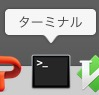
\includegraphics[scale=0.5]{./Figure/elementaryCS-figTermIcon.jpg}
  \end{center}
\end{frame}
\begin{frame}[containsverbatim]
\frametitle{プログラム開発の流れ}
  \begin{center}
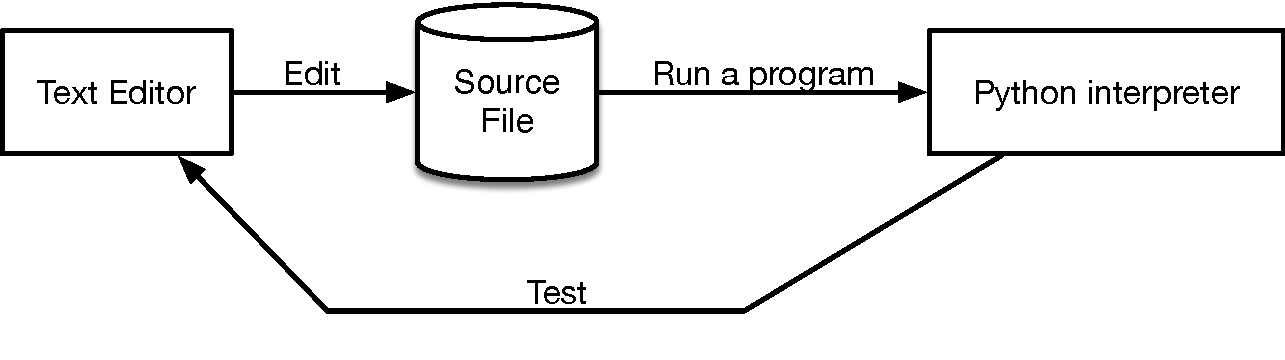
\includegraphics[scale=0.3]{./Figure/CS-figEditAndRun.pdf}
  \end{center}
\end{frame}
\begin{frame}[fragile]
\frametitle{ターミナルを使ってみよう}
  \begin{itemize}
\item ターミナルを使ってプログラムを実行してみよう
\item Terminal を起動
\item コマンドプロンプト \verb|>| が表示されたらホームディレクトリの下に適当なディレクトリ (例えば CS1) を作成
\item \href{https://sites.google.com/presystems.xyz/elementarycs/top}{\beamerbutton{https://sites.google.com/presystems.xyz/elementarycs/top}} から必要なファイル (gcd.py) を作成したディレクトリにダウンロード
    \begin{itemize}
\item ホームディレクトリの下の Downloads に保存されるかも
    \end{itemize}
  \end{itemize}
  \begin{itembox}{準備}
\scriptsize
    \begin{verbatim}
> mkdir CS1       # 課題用のディレクトリを作成
> cd CS1          # 課題用ディレクトリに移動
> python3 gcd.py  # プログラムを実行
    \end{verbatim}
  \end{itembox}
\end{frame}
%
%%% EDIT SROURCE FILE
%
\subsection{ソースファイルの編集}
\begin{frame}[containsverbatim]
\frametitle{ソースファイルの編集}
  \begin{itemize}
\item テキストエディタと呼ばれるソフトウェアを使って編集
    \begin{itemize}
\item vim, emacs など
    \end{itemize}
\item ターミナルからコマンド入力して起動
  \end{itemize}
  \begin{itembox}{editor の起動}
\scriptsize
    \begin{verbatim}
> open -a Emacs gcd.py
あるいは
> open -a Macvim gcd.py
    \end{verbatim}
  \end{itembox}
\end{frame}
%
%%% Run a Program
%
%\subsection{プログラムを走らせてみる}
%\begin{frame}[containsverbatim]
%\frametitle{プログラムを走らせてみる}
%  \begin{itemize}
%\item コマンドプロンプト \verb|>| が表示されたら phtyon3 とソースファイル名と入力して return 
%\item Python プログラムが実行されます
%  \end{itemize}
%  \begin{columns}
%    \begin{column}{0.5\textwidth}
%      \begin{itembox}{\footnotesize Python の起動}
%\scriptsize
%        \begin{verbatim}
%> python3 sub.py
%        \end{verbatim}
%      \end{itembox}
%    \end{column}
%    \begin{column}{0.5\textwidth}
%      \begin{itembox}{\footnotesize Ruby の起動と終了}
%\scriptsize
%        \begin{verbatim}
%> irb
%>> load smile.rb
%>> quit
%        \end{verbatim}
%      \end{itembox}
%    \end{column}
%  \end{columns}
%\end{frame}

%
%%% 計算の基本
%
\part{計算の基本}
\frame{
  \frametitle{計算の基本}
\scriptsize
  \tableofcontents[part=2]
}
\section{はじめに}
%
%%% GOAL
%
\subsection{課題 1 の目標とテーマ}
\begin{frame}
\frametitle{課題 1の目標とテーマ}
  \begin{columns}
    \begin{column}{0.6\textwidth}
      \begin{itemize}
\item 目標
        \begin{itemize}
\item 計算の基本要素を知る
        \end{itemize}
\item テーマ
        \begin{itemize}
\item 四則演算でアニメーション
\item \movie[once,externalviewer]{\beamerbutton{ひつじさん}}{./Figure/sheep-python.mov}
        \end{itemize}
      \end{itemize}
    \end{column}
    \begin{column}{0.4\textwidth}
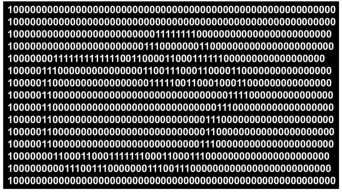
\includegraphics[scale=0.6]{./Figure/sheep-fixed.pdf}
    \end{column}
  \end{columns}
\end{frame}
\subsection{CS のこころ}
\begin{frame}
\frametitle{CS のこころ}
  \begin{itemize}
\item しつこいようですが,すべては計算
\item コンピュータに載せるには
    \begin{itemize}
\item 対象をデータとして表すこと
\item 処理を基本演算の組み合わせで表すこと
    \end{itemize}
\item 処理とはコンピュータのなかの抽象的な世界に存在して
\item データというもう一つの抽象的な存在を操作する
\item この処理やデータをプログラミング言語の記号をもちいて注意深く構成したのがプログラム
  \end{itemize}
\end{frame}
%
%%% What's DATA
%
\section{データは数である}
\begin{frame}
\frametitle{データは数である}
  \begin{itemize}
\item データから見ていくことにして
\item データはすべて 2 進列で表される
    \begin{itemize}
\item 自然数,整数,実数: 18, -3, 3.14 など
\item 文字: 文字コード: ASCII, Unicode など
\item 画像,映像
\item 音
\item におい,味,触覚
    \end{itemize}
  \end{itemize}
\end{frame}
%
%%% Number
%
\subsection{Bit と Byte}
\begin{frame}
\frametitle{情報とは}
  \begin{itemize}
\item ここで情報とは何か考えてみます
\item 情報とは"ある物事,事情についてのお知らせ"
\item 情報の価値はどう決まるか?
    \begin{itemize}
\item 驚きをもって受け止められる情報は価値が高い?
\item 日常的な情報は価値が低い?
    \end{itemize}
  \end{itemize}
\end{frame}
\begin{frame}
\frametitle{まずは情報量というもの}
  \begin{enumerate}
\item ある結果や情報を得る場合を考える
\item 結果や情報を生じる事象が確率現象であると見なす
\item 確率 $p$ の事象の情報量を \(I(p)\) であらわす
\item \(I(p)\) は単調減少関数
    \begin{itemize}
\item 頻繁に起こっていること ((\(p\) が大きい) は情報量が少ない)
\item 頻繁に起こらないこと ((\(p\) が小さい) は情報量が多い)
    \end{itemize}
\item 連続関数である
    \begin{itemize}
\item 確率のわずかな変化で情報量が大きく変化するのは不自然
    \end{itemize}
  \end{enumerate}
  \begin{block}{情報量の定義}
ある事象 $a$ の生起確率を \(p_a\) とすると
その情報量 \(I(p_a)\) は \(\log_{2}\frac{1}{p_a}=-\log_{2}p_a\) であらわすことにする
  \end{block}
\end{frame}
\begin{frame}
\frametitle{ビットとは}
  \begin{block}{1 bit とは}
    \begin{enumerate}
\item 今, 2 つの事象を考える
\item 同じ確率 \(P=\frac{1}{2}\) で生起するとする
\item このとき,ひとつの事象 $a$ の情報量 \(I(a)=\log_2\frac{1}{\frac{1}{2}}=1\)
\item これが 1 bit
\item 確率 \(\frac{1}{2}\) で起こる事象を知った時の情報量が 1 bit(ビット)
    \end{enumerate}
  \end{block}
  \begin{itemize}
\item それでは確率 \(\frac{1}{10}\) で起こる事象を知った時は 1 hartley(ハートレー)
\item 確率 \(\frac{1}{e}\) では 1 nat(ナット)
  \end{itemize}
\end{frame}
\begin{frame}
\frametitle{情報の記録}
  \begin{itemize}
\item 情報はビットの列として記録
\item 明確に区別された 2 つの状態で記録しています
    \begin{itemize}
\item 磁性体の向き,電圧の高低,スイッチの開閉
    \end{itemize}
\item 計算機科学では 2 つの状態を便宜的に $0$ と $1$ として議論しています
  \end{itemize}
\end{frame}
\begin{frame}
\frametitle{ビットによる表現}
  \begin{itemize}
\item 2 つの状態を取り得るデバイスを $N$ 個並べてそれぞれ独立としたらどれだけの情報があらわせるか
\item 答えは \(\log_2 2^N=N\) となり $N$ ビットの情報量となります
\item $N$ ビットでどれだけの事象を区別できるでしょうか
\item 答えは 2 個の要素から $N$ 個の重複順列 \({ }_2\Pi_N=2^N\) です
  \end{itemize}
\end{frame}
\begin{frame}
\frametitle{バイトとは}
  \begin{itemize}
\item 人間にとって意味をなす長さ $N$ の小ブロック
\item 現在のコンピュータでは 8 bit としています
  \end{itemize}
\end{frame}
%
%%% Number
%
\subsection{自然数の n 進表記}
\begin{frame}
\frametitle{数表記}
  \begin{itemize}
\item ビットの列で表すことは先に述べました
\item では自然数はどうあらわすでしょう
\item 数表記は 10 進が唯一の方法ではありません
\item $n$ 進表記が可能です
\item 数はどうコンピュータ内で表現されるかみていきます
  \end{itemize}
\end{frame}
\begin{frame}
\frametitle{$n$ 進表記}
  \begin{itemize}
\item 実は日常的に $n$ 進法を利用しています
\item 時間は 24 進法, 60 進法, 30 進法,360 進法をもちいています
\item たとえば 24 進法では 24 になったら位が一つ上がります
\item コンピュータでは 2 進法をもちいて自然数を表します
\item 2 進法ではやはり人間には分かりずらいので 8 進法や 16 進法であらわすことが多いです
  \end{itemize}
\end{frame}
\begin{frame}
\frametitle{$n$ 進法の各桁}
  \begin{itemize}
\item 2 進法,8 進法,16 進法でも 10 進法と同じように位どりによってあらわします
\item 良くご存知のように 10 進法では 1 桁を 0-9 のいづれかであらわしています
\item 123 という自然数であれば \(1\times 10^2+2\times 10^1+3\times 10^0\) といった具合です
  \end{itemize}
\end{frame}
\begin{frame}
\frametitle{2 進法の各桁}
  \begin{itemize}
\item 2 進法では各桁は 0 と 1 だけになります
\item 10 進法の場合と同様に位どりします,ただし底が 2 になります
\item \((010)_2\) という自然数であれば \(0\times 2^2+1\times 2^1+0\times 2^0\) といった具合です
\item この例では \((2)_{10}\) は位が一つ上がって \((010)_2\) となっています
  \end{itemize}
\end{frame}
\begin{frame}
\frametitle{16 進法の各桁}
  \begin{itemize}
\item 2 進法では桁が多くなって見ずらいので 16 進で表記します
\item 16 進法では各桁:
    \begin{itemize}
\item 0,1,2,3,4,5,6,7,8,9 と 0-9 までは 10 進と同じ
\item 10,11,12,13,14,15 は A,B,C,D,E,F をもちいます
    \end{itemize}
\item 10 進法の場合と同様に位どりします,ただし底が 16 になります
\item \((1F0)_{16}\) という自然数であれば \(1\times 16^2+F\times 16^1+0\times 16^0\) といった具合です
  \end{itemize}
\end{frame}
\begin{frame}
\frametitle{各数字の対応}
  \begin{columns}[t]
    \begin{column}{5cm}
\footnotesize
      \begin{tabular}{c|c|c|c}
10 進 & 8 進 & 16 進 & 2 進\\
\hline
 0& 0& 0&0\\
 1& 1& 1&1\\
 2& 2& 2&10\\
 3& 3& 3&11\\
 4& 4& 4&100\\
 5& 5& 5&101\\
 6& 6& 6&110\\
 7& 7& 7&111\\
      \end{tabular}
    \end{column}
    \begin{column}{5cm}
\footnotesize
      \begin{tabular}{c|c|c|c}
10 進 & 8 進 & 16 進 & 2 進\\
\hline
 8&10& 8&1000\\
 9&11& 9&1001\\
10&12& A&1010\\
11&13& B&1011\\
12&14& C&1100\\
13&15& D&1101\\
14&16& E&1110\\
15&17& F&1111\\
      \end{tabular}
    \end{column}
  \end{columns}
\end{frame}
\begin{frame}[label=Dec2Bin]
\frametitle{$n$ 進数の変換}
  \begin{itemize}
\item $m$ 進数から $n$ 進数への変換
\item 手始めに 10 進数から 2 進数への変換
  \end{itemize}
  \begin{center}
   \begin{example}[10進$\Leftrightarrow$2進]
   \begin{columns}[t]
    \begin{column}{3cm}
\infer[\mbox{High}]{0}{\infer{2)1\cdots 1}{\infer{2)2\cdots 0}{\infer{2)4\cdots 0}{\infer[\mbox{Low}]{2)9\cdots 1}{2)19\cdots 1}}}}}
    \end{column}
    \begin{column}{3cm}
\infer{19}{\infer{1\times 2^4=16}{\infer{0\times 2^3=0}{\infer{0\times 2^2=0}{\infer{1\times 2^1=2}{1\times 2^0=1}}}}}
    \end{column}
   \end{columns}
   \end{example}
  \end{center}
\end{frame}
\begin{frame}
\frametitle{Quiz: 10 進表記$\Leftrightarrow$ 2 進表記 の変換}
  \begin{block}{Quiz}
    \begin{enumerate}
\item 131$_{10}$, 112$_{10}$ を 2 進数に変換してみてください\label{lb:first}
\item \ref{lb:first}で得られた 2 進数を 10 進表記に戻してください
\item もとの 10 進数が得られれば正しく変換できています
\item この数字は東工大に割り当てられた IP アドレスになります
    \end{enumerate}
  \end{block}
\end{frame}
%\section{数の表現}
\begin{frame}[shrink]
\frametitle{繰り返しや再帰によるその他の計算}
  \begin{itemize}
\item 繰り返しや再帰は自然数 $n$ に対応する解を求めるような感じ
    \begin{itemize}
\item 数列は $n$ 番目の数を求める: \(\alpha\colon N\rightarrow N\)
\item ハノイの塔も $n$ 枚目の解を求める
    \end{itemize}
\item これを利用して関数の解を求める計算に利用する
\item たとえば非線形方程式 \(f(x)=0\) の実根を求める
\item \href{run:newton.command}{\beamerbutton{ニュートン法}}
    \begin{itemize}
\item \(\sqrt{a}\) を求めてみる
\item \(f(x)=x^2-a\) として \(f(x)=0\) となる $x$ を求める
\item \(k+1\) 番目の近似値 \(x_{k+1}\) を
      \begin{displaymath}
x_{k+1} = x_k-\frac{f(x_k)}{f'(x_k)} = \frac{1}{2}(x_k+\frac{a}{x_k})
      \end{displaymath}
で求める
\item \(x_{k+1}\) と \(x_k\) が十分近くなったら停止
    \end{itemize}
  \end{itemize}
\end{frame}
\subsection{非負整数の表現}
\begin{frame}[label=Top_Integer]
\frametitle{非負整数のコンピュータ内での表現}
  \begin{itemize}
\item 10 進数から 2 進数への変換
  \end{itemize}
  \begin{center}
   \begin{example}[10進$\Leftrightarrow$2進]
   \begin{columns}[t]
    \begin{column}{3cm}
\infer[\mbox{High}]{0}{\infer{2)1\cdots 1}{\infer{2)2\cdots 0}{\infer{2)4\cdots 0}{\infer[\mbox{Low}]{2)9\cdots 1}{2)19\cdots 1}}}}}
    \end{column}
    \begin{column}{3cm}
\infer{19}{\infer{1\times 2^4=16}{\infer{0\times 2^3=0}{\infer{0\times 2^2=0}{\infer{1\times 2^1=2}{1\times 2^0=1}}}}}
    \end{column}
   \end{columns}
   \end{example}
  \end{center}
\end{frame}
\subsection{負の数の表現}
\begin{frame}[shrink]
\frametitle{負の数の表現}
  \begin{itemize}
\item 負の数をあらわすには補数表現をもちいます
\item それでは 2 の補数(2's complement) を求めてみましょう
  \end{itemize}
  \begin{block}{2 の補数表現}
    \begin{enumerate}
\item 2 進表記において各ビットを反転する
\item それに 1 を足す
    \end{enumerate}
  \end{block}
  \begin{center}
    \begin{example}[-8$\sim$7 (2 進 4 桁) の 2 の補数表現]
\((1000)_{(2)}\Rightarrow(1001)_{(2)}\Rightarrow(1010)_{(2)}\Rightarrow (1011)_{(2)}\Rightarrow (1100)_{(2)}
\Rightarrow(1101)_{(2)}\Rightarrow(1110)_{(2)}\Rightarrow(1111)_{(2)}
\Rightarrow(0000)_{(2)}\Rightarrow(0001)_{(2)}\Rightarrow(0010)_{(2)}\Rightarrow(0011)_{(2)}
\Rightarrow(0100)_{(2)}\Rightarrow(0101)_{(2)}\Rightarrow(0110)_{(2)}\Rightarrow(0111)_{(2)}\)\\
      \begin{itemize}
\item Successor (1 足す) でつぎの数になるようになっている
\item 最上位ビットがサインビットになっている
\item circulation の実行
      \end{itemize}
    \end{example}
  \end{center}
\end{frame}
\subsection{計算機内の計算}
\begin{frame}[shrink]
\frametitle{計算機内の計算}
\framesubtitle{整数の減算}
  \begin{itemize}
\item 2 進 $n$ 桁の数 $a, b$ (\(A_k,B_k\in\{1,0\}\))
    \begin{itemize}
\item \(a\colon A_{n-1}A_{n-2}\cdots A_{1}A_{0}\)
\item \(b\colon B_{n-1}B_{n-2}\cdots B_{1}B_{0}\)
    \end{itemize}
\item \(a, b\) はそれぞれ
\[a=\sum_{k=0}^{n-1}2^{k}A_{k}\]
\[b=\sum_{k=0}^{n-1}2^{k}B_{k}\]
\item $b$ の各桁を反転させたものを \(\overline{B_{k}}\) として $b$ の補数 \(\overline{b}\) は
\[\overline{b}=\sum_{k=0}^{n-1}2^{k}\overline{B_{k}}=\sum_{k=0}^{n-1}2^{k}(1-B_{k})=(2^n-1)-b\]
  \end{itemize}
\end{frame}
\begin{frame}[shrink]
\frametitle{計算機内の計算\textemdash Cont.}
  \begin{itemize}
\item \(\overline{b}=(2^n-1)-b\) より
    \begin{eqnarray*}
a-b&\Rightarrow& a-((2^n-1)-\overline{b})\\
   &=&a+\overline{b}+1-2^n
    \end{eqnarray*}
\item 引き算は補数を足すことで表す
\item \(\overline{b}+1\) は 2 の補数
\item \(-2^n\) は最上位の桁上がりは無視
  \end{itemize}
  \begin{example}[引き算の例]
    \begin{itemize}
\item 4 桁の2進数と仮定して \(6-3\) と \(3-6\)
    \end{itemize}
    \begin{columns}[t]
      \begin{column}{3.5cm}
        \begin{tabular}{ccccc}
&0&1&1&0\\
$+$&1&1&0&1\\
\hline
&0&0&1&1\\
        \end{tabular}
      \end{column}
      \begin{column}{3.5cm}
        \begin{tabular}{ccccc}
&0&0&1&1\\
$+$&1&0&1&0\\
\hline
&1&1&0&1\\
        \end{tabular}
      \end{column}
    \end{columns}
  \end{example}
\end{frame}

%\subsection{実数の表現}
\begin{frame}[shrink]
\frametitle{実数の表現}
\framesubtitle{浮動小数 (floating point number)}
  \begin{itemize}
\item 浮動小数 \(ab^{e}\)
    \begin{itemize}
\item $a$ は仮数 (significand or coefficient) ,$b$ は底 (base),$e$ は指数 (exponent) と呼ぶ
    \end{itemize}
\item \(\frac{1}{b}\leq|a|<1\) のとき正規浮動小数 (normalized floating point number) と云う
\item 上のような変換を正規化(normalizaiton) と云う
\item 符号,指数,仮数で一意に決定できます
  \end{itemize}
  \begin{example}[正規浮動小数]
   \begin{math}
    \begin{array}{rcl}
1.234 &\Rightarrow& +0.1234\times 10^1\\
-12.34 &\Rightarrow& -0.1234\times 10^2\\
0.01234 &\Rightarrow& +0.1234\times 10^{-2}\\
    \end{array}
   \end{math}
  \end{example}
\end{frame}
\begin{frame}
\frametitle{実数の 2 進表記}
  \begin{itemize}
\item 実数も 2 進表記に変換した上で正規化します
\item 13.6875$_{(10)}$ を2進数へ変換してみます
  \end{itemize}
  \begin{center}
   \begin{example}[10進実数 13.6875$_{(10)}$ を2進数へ]
     \begin{columns}[t]
       \begin{column}{4.5cm}
\infer[High]{0}{\infer{2)1\cdots 1}{\infer{2)3\cdots 1}{\infer[Low]{2)6\cdots 0}{2)13\cdots 1}}}}
         \begin{itemize}
\item 13$_{(10)}$ は 1101$_{(2)}$
         \end{itemize}
       \end{column}
     \begin{column}{4.5cm}
\infer[Low]{.5\times 2=1.00}{\infer{.75\times 2=1.50}{\infer[High]{.375\times 2=0.75}{.6875\times 2=1.375}}}
     \begin{itemize}
\item .6875$_{(10)}$ は .1011$_{(2)}$
     \end{itemize}
      \end{column}
     \end{columns}
     \begin{itemize}
\item ゆえに, 13.6875$_{(10)}$ は 1101.1011$_{(2)}$ となる 
     \end{itemize}
   \end{example}
  \end{center}
\end{frame}
\begin{frame}
\frametitle{実数の 2 進表記 - Cont.}
  \begin{itemize}
\item 得られた 2 進数を正規化します
\item 最上位ビットが 1 になるようにします (注意: 正規化の定義と違っているので注意)
  \end{itemize}
  \begin{center}
    \begin{example}[1101.1011$_{(2)}$ を正規化]
1101.1011$_{(2)}$ \(\Rightarrow\) 0.11011011\(\times 2^4\)
      \begin{itemize}
\item 符号: +
\item 指数: 4
\item 仮数: 0.11011011
      \end{itemize}
    \end{example}
  \end{center}
\end{frame}
\begin{frame}[shrink]
\frametitle{実数の 2 進表記 - Cont.}
  \begin{itemize}
\item 符号,指数,仮数が正規化によって決まります
\item これを 32 ビットで表す
\item 右に小数点を一つ移動
\item 最上位ビットは必ず 1 になるので省略
\item 規格 \href{http://ieeexplore.ieee.org/xpl/mostRecentIssue.jsp?punumber=2355}{\beamerbutton{IEEE 754}} はもうひと段階
  \end{itemize}
  \begin{center}
    \begin{example}[指数部,仮数部]
      \begin{itemize}
\item 1.1011011\(\times 2^3\) の符号,指数,仮数は以下のとおり
        \begin{itemize}
\item 符号 (sign): +
\item 指数 (exponent): 3
\item 仮数 (significand): 1.1011011
        \end{itemize}
      \end{itemize}
    \end{example}
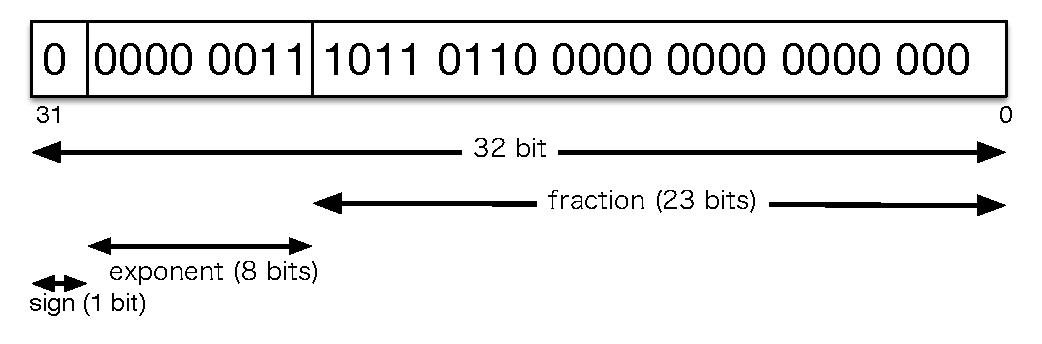
\includegraphics[scale=.4]{./Figure/elementaryCS-figFloatingPointFormat.eps}
  \end{center}
\end{frame}
\begin{frame}
\frametitle{宿題 3: 浮動小数}
  \begin{itemize}
\item 実数の浮動小数表現をやってみてください
  \end{itemize}
  \begin{block}{宿題 3}
    \begin{itemize}
\item 35.75 を浮動小数で表現してみてください
\item T2Schola に小テストがあるのでそれに答えてください
    \end{itemize}
  \end{block}
\end{frame}
\begin{frame}
\frametitle{宿題 3: 回答}
  \begin{itemize}
\item 2 進へ変換: 100011.11
\item 正規化: 1.0001111$\times 2^5$
\item 32 bit 形式に: {\scriptsize 0 0000 0101 0001 1110 0000 0000 0000 000}
    \begin{itemize}
\item 1. は省略
    \end{itemize}
\item 規格\href{http://ieeexplore.ieee.org/xpl/mostRecentIssue.jsp?punumber=2355}{\beamerbutton{IEEE 754}}では下駄 (bais) をはかせるので\(5+127=132\Rightarrow\) 1000 0100
\item 32 bit 形式に: {\scriptsize 0 1000 0100 0001 1110 0000 0000 0000 000}
  \end{itemize}
\end{frame}
\subsection{浮動小数の算術演算}
\begin{frame}[shrink,fragile]
\frametitle{浮動小数演算の変な現象 1}
  \begin{itemize}
\item roundoff.py を実行してみます
\item 結果が予測と少し違うことになります
\item \(0.6_{(10)}\) は \((0.1001\ldots)_{(2)}\), \(0.4_{(10)}\) は \((0.0110\ldots)_{(2)}\), \(0.2_{(10)}\) は \((0.0011\ldots)_{(2)}\) となります
  \end{itemize}
  \begin{lstlisting}[caption={roundoff.py},label=lst:roundoff]
if (float(0.6)-float(0.4)==float(0.2)):
   print("is equal")
else:
   print("not equal")
  \end{lstlisting}
\end{frame}
\begin{frame}[shrink,fragile]
\frametitle{浮動小数演算の変な現象 2}
  \begin{itemize}
\item machine\_epsilon.py を実行してみます
\item 結果が予測と少し違うことになります
\item この原因についてみていきます
  \end{itemize}
  \begin{lstlisting}[caption={machine\_epsilon.py},label=lst:epsilon]
# Machine epsilon
import sys

epsilon, old, prod =1.0, 0.0, 0.0
cnt=0
while (prod!=1.0):
  print(epsilon)
  old = epsilon
  cnt=cnt+1
  epsilon=epsilon/2.0
  prod=epsilon+1.0
print("Calculated machine epsilon:",old)
print("System information in Python:",sys.float_info.epsilon)
  \end{lstlisting}
\end{frame}
\begin{frame}[shrink]
\frametitle{浮動小数数の算術演算}
  \begin{itemize}
\item 正規化した 2 つの浮動小数 \(X, Y\) を \(X=F_x\times 10^{e_x}, Y=F_y\times 10^{e_y}\) とする
\item 乗算: \(XY=(F_x\times 10^{e_x})(F_y\times 10^{e_y})=F_xF_y\times 10^{e_x+e_y}\)
\item 除算: \(\frac{X}{Y}=\frac{(F_x\times 10^{e_x})}{(F_y\times 10^{e_y})}=\frac{F_x}{F_y}\times 10^{e_x-e_y}\)
\item 加算\(\cdot\)減算: \(X\pm Y=(F_x\times 10^{e_x})\pm(F_y\times 10^{e_y})=(F_x\pm F_y\cdot 10^{e_y-e_x})\times 10^{e_x}\)
    \begin{itemize}
\item ただし,\(e_x\geq e_y\)
\item \(F_y\cdot 10^{e_y-e_x}\) は指数を大きい方に揃えたときの $Y$ の仮数
    \end{itemize}
\item 演算結果も正規化するので指数は調整が必要
  \end{itemize}
  \begin{example}[算術演算の例]
    \begin{columns}[t]
      \begin{column}{4.5cm}
        \begin{math}
          \begin{array}{cll}
&0.2184&\times 10^2\\
\times&0.2512&\times 10^2\\
\hline
&0.07998208&\times 10^4\\
=&0.7998208&\times 10^3\\
          \end{array}
        \end{math}
      \end{column}
      \begin{column}{4.5cm}
        \begin{math}
          \begin{array}{cll}
&0.2844&\times 10^3\\
+&0.4162&\times 10^1\\
\hline
&0.288562&\times 10^3\\
          \end{array}
        \end{math}
      \end{column}
    \end{columns}
  \end{example}
\end{frame}
%\begin{frame}
%\frametitle{算術演算の誤差}
%  \begin{itemize}
%\item 4 桁までしか記憶できないと仮定
%\item \(0.2844\cdot 10^3+0.4162\cdot 10^1=0.288562\cdot 10^3=(0.2885+0.000062)\cdot 10^3=0.2885\cdot 10^3+0.6200\cdot 10^{-1}\)
%\item \(0.288562\)が真の値となるが \(0.2885\) までしか記憶できないので
%\item \(0.6200\cdot 10^{-1}(=0.000062\cdot 10^3)\) について調整する必要がある
%  \end{itemize}
%  \begin{example}[\(0.2844\cdot 10^3+0.4162\cdot 10^1\)]
%    \begin{columns}[t]
%      \begin{column}{4.5cm}
%        \begin{math}
%          \begin{array}{cll}
%&0.2844&\times 10^3\\
%+&0.4162&\times 10^1\\
%\hline
%&0.288562&\times 10^3\\
%          \end{array}
%        \end{math}
%      \end{column}
%      \begin{column}{4.5cm}
%        \begin{math}
%          \begin{array}{cll}
%&0.2844&\times 10^3\\
%+&0.004162&\times 10^3\\
%\hline
%&0.288562&\times 10^3\\
%          \end{array}
%        \end{math}
%      \end{column}
%    \end{columns}
%  \end{example}
%\end{frame}
\section{誤差のおはなし}
\subsection{丸め誤差 (roundoff error)}
\begin{frame}[shrink]
\frametitle{誤差とは}
  \begin{itemize}
\item コンピュータの中では実数は有限個の 0 と 1 の組み合わせ(浮動小数)で表しています
\item なので,本来あるべき真値を適当な浮動小数で近似している
\item 近似値-真値 を誤差という
  \end{itemize}
\end{frame}
\begin{frame}[shrink]
\frametitle{丸め誤差 (roundoff error)}
  \begin{itemize}
\item 表現可能な範囲に丸めることを丸め誤差という(\lstref{lst:roundoff}参照)
\item 演算結果も丸める
\item $Z$ を演算結果とする
\item $d$ 桁だけ記憶できるとして,先頭の $d$ 桁を $F$,残りを $f$ とすると,\(Z=F\cdot 10^{e_z}+f\cdot 10^{e_z-d}\)
\item $f$ の値で四捨五入することにして
    \begin{displaymath}
      \begin{array}{ll}
|f|<0.5 \mbox{のとき} & |Z|=|F|\cdot 10^{e_z-d}\\
|f|\geq 0.5 \mbox{のとき} & |Z|=|F|\cdot 10^{e_z-d}+\cdot 10^{e_z-d}
      \end{array}
    \end{displaymath}
\item 丸め誤差 $\epsilon_z$ とすれば
    \begin{displaymath}
      \begin{array}{ll}
|f|<0.5 \mbox{のとき} & |\epsilon_z|=|f|\cdot 10^{e_z-d}\\
|f|\geq 0.5 \mbox{のとき} & |\epsilon_z|=|1-f|\cdot 10^{e_z-d}
      \end{array}
    \end{displaymath}
  \end{itemize}
  \begin{example}[\(0.2844\cdot 10^3+0.4162\cdot 10^1\)]
    \begin{itemize}
\item \(0.2844\cdot 10^3+0.4162\cdot 10^1=0.2885\cdot 10^3+0.6200\cdot 10^{-1}\)
\item \(|Z|=0.2885\cdot 10^3+10^{3-4}=0.2886\cdot 10^3\)
\item \(|\epsilon_z|=|1-0.6200|\cdot 10^{3-4}=0.48\cdot 10^{-1}\)
    \end{itemize}
  \end{example}
\end{frame}
%\begin{frame}
%\frametitle{相対誤差 (relative error)}
%  \begin{itemize}
%\item 計算のコストだけでなくときには計算精度も重要になる
%\item 真の値 $x^t$,観測した値 $x$ として誤差 \(\epsilon_x=x^t-x\)
%\item \(|\epsilon_x|=|x^t-x|\) を絶対誤差という
%\item 相対誤差 \(r_x=\frac{\epsilon_{x}}{x}=\frac{x^t-x}{x}\) で精度を測る
%  \end{itemize}
%  \begin{example}[相対誤差の例]
%    \begin{itemize}
%\item \(x_t=9, x=10\) と \(y_t=999, y=1000\) の場合を考える
%\item $x$ と $y$ の誤差はどちらも \(-1\)
%\item $x$ と $y$ の相対誤差はそれぞれ \(r_x=\frac{-1}{10}, r_y=\frac{-1}{1000}\)
%    \end{itemize}
%  \end{example}
%\end{frame}
%\subsection{誤差の伝搬 (propagation of errors)}
%\begin{frame}
%\frametitle{誤差の伝搬 (propagation of errors)}
%  \begin{itemize}
%\item 誤差は計算中伝播して計算結果を不正確にしてしまう
%\item 算術式中の誤差がどう蓄積されていくかをみる
%\item ある数 $x, y$ としてそれぞれが誤差 \(\epsilon_x, \epsilon_y\) を持つとする
%\item このときの演算 \(x\oplus y\) の誤差 \(\epsilon_{x\oplus y}\) は
%    \begin{displaymath}
%\epsilon_{x\oplus y}=(x^t\oplus y^t)-(x\oplus y)
%    \end{displaymath}
%\item \(x^t\oplus y^t\) は真の演算結果で, \(x\oplus y\) は実際の結果
%\item 先の誤差の定義からこれが導ける
%  \end{itemize}
%\end{frame}
%\begin{frame}[shrink]
%\frametitle{誤差公式}
%  \begin{itemize}
%\item 各演算についてつぎの関係が成り立つ
%  \end{itemize}
%  \begin{theorem}[誤差公式]
%    \begin{math}
%      \begin{array}{lclclclcl}
%\scriptsize
%\epsilon_{x+y}&=&(x^t+y^t)-(x+y)&=&(x^t-x)+(y^t-y)&=&\epsilon_x+\epsilon_y\\
%\epsilon_{x-y}&=&(x^t-y^t)-(x-y)&=&(x^t-x)-(y^t-y)&=&\epsilon_x-\epsilon_y\\
%      \end{array}
%    \end{math}
%    \begin{math}
%      \begin{array}{lclclclcl}
%\epsilon_{xy}&=&(x^ty^t)-(xy)&=&(x+\epsilon_x)(y+\epsilon_y)-(xy)&=&\epsilon_x y+\epsilon_y x\\
%      \end{array}
%    \end{math}
%    \begin{math}
%      \begin{array}{lclclclcl}
%\epsilon_{\frac{x}{y}}&=&\frac{x^t}{y^t}-\frac{x}{y}&=&\frac{x^ty-y^tx}{y^ty}&=&\frac{(x+\epsilon_x)y-(y+\epsilon_y)x}{(y+\epsilon_y)y}\\
%&=&\frac{xy+\epsilon_xy-xy+x\epsilon_y}{y^2(1+\frac{\epsilon_y}{y})}&=&\frac{\epsilon_xy-\epsilon_yx}{y^2}\\
%      \end{array}
%    \end{math}
%    \begin{itemize}
%\item \(\epsilon_x\epsilon_y\) は十分小さいとして無視
%\item \(|\frac{\epsilon_y}{y}|\) は \(|\frac{\epsilon_y}{y}|\ll 1\) のとき無視
%\item これに各演算の丸め誤差 \(\alpha\) を加えたて誤差公式とする
%      \begin{itemize}
%\item たとえば 4 桁までしか記憶できないのであれば演算結果も 4 桁に丸められる
%      \end{itemize}
%    \end{itemize}
%  \end{theorem}
%\end{frame}
%\begin{frame}[shrink]
%\frametitle{相対誤差公式}
%  \begin{itemize}
%\item 相対誤差公式を導く
%\item 先の相対誤差の定義より
%    \begin{displaymath}
%r_{x\oplus y}=\frac{\epsilon_{x\oplus y}}{x\oplus y}
%    \end{displaymath}
%\item とすれば誤差公式よりつぎの相対誤差公式をえる
%  \end{itemize}
%  \begin{theorem}[相対誤差公式]
%    \begin{math}
%      \begin{array}{rclcl}
%r_{x+y}&=&\frac{\epsilon_x+\epsilon_y}{x+y}+\alpha&=&r_x\frac{x}{x+y}+r_y\frac{y}{x+y}+\alpha\\
%r_{x-y}&=&\frac{\epsilon_x-\epsilon_y}{x-y}+\alpha&=&r_x\frac{x}{x-y}+r_y\frac{-y}{x-y}+\alpha\\
%r_{xy}&=&\frac{\epsilon_x y+\epsilon_y x}{xy}+\alpha&=&r_x\ 1+r_y\ 1+\alpha\\
%r_{xy}&=&\frac{\frac{\epsilon_x y-\epsilon_y x}{y^2}}{\frac{x}{y}}+\alpha&=&r_x\ 1+r_y\ (-1)+\alpha
%      \end{array}
%    \end{math}
%  \end{theorem}
%\end{frame}
%\begin{frame}[shrink]
%\frametitle{誤差伝播の解析}
%  \begin{itemize}
%\item 相対誤差公式を使って誤差伝播の解析を行う
%  \end{itemize}
%  \begin{example}[和における誤差伝播]
%    \begin{itemize}
%\item \(r_0, r_1, r_2, r_3\) を実数 \(a_0,a_1,a_2,a_3\) の相対誤差とする
%\item \(S=(((a_0+a_1)+a_2)+a_3)\) の相対誤差を求める
%    \end{itemize}
%  \end{example}
%\end{frame}
\subsection{情報落ち誤差}
\begin{frame}[shrink]
\frametitle{情報落ち誤差(loss of trailing digits)}
  \begin{itemize}
\item 絶対値が大きく異なる 2 つの数の加減算では小さい数が無視されることがある
\item \lstref{lst:epsilon} で見たような場合
  \end{itemize}
\end{frame}
\subsection{打ち切り誤差 (truncation error)}
\begin{frame}[shrink]\label{sl:back}
\frametitle{打ち切り誤差 (truncation error)}
  \begin{itemize}
\item コンピュータでは無限に繰り返して値をもとめることはできない
\item 有限回の計算で値を計算し,それを求める値の近似値としてもちいる
\item このときの誤差を打切り誤差という
  \end{itemize}
  \begin{example}[\(\sin(x)\)のマクローリン展開]
    \begin{itemize}
\item \(sin(x)=x-\frac{x^3}{3!}+\frac{x^5}{5!}-\frac{x^7}{7!}+\cdots+(-1)^{n}\frac{x^{2n+1}}{(2n+1)!}+\cdots\)
\item gnuplot で試してみてください
    \end{itemize}
  \end{example}
  \begin{example}[平方根の計算]
    \begin{itemize}
%\item \href{run:newton.command}{\beamerbutton{ニュートン法}}
\item newton.py を参照\hyperlink{newton-is_enough-rec}{\beamerbutton{プログラム例}}
\item \(\sqrt{a}\) を求めてみる
\item \(f(x)=x^2-a\) として \(f(x)=0\) となる $x$ を求める
\item \(k+1\) 番目の近似値 \(x_{k+1}\) を
      \begin{displaymath}
x_{k+1} = x_k-\frac{f(x_k)}{f'(x_k)} = \frac{1}{2}(x_k+\frac{a}{x_k})
      \end{displaymath}
    \end{itemize}
  \end{example}
\end{frame}
%\section{まとめ}
%\begin{frame}[shrink,fragile]
%\frametitle{数値計算}
%  \begin{itemize}
%\item ここで取り上げたおはなしは数値計算(計算機科学の一分野)のなかの計算誤差をとりあげたもの
%\item シミュレーションなどではある関数の実際の数値を必要とする場合がある
%    \begin{itemize}
%\item 例えば,方程式 \(f(x)=0\) の $x$ を数値的に求める
%    \end{itemize}
%\item 数値計算の手順
%    \begin{itemize}
%\item 最初に適当な 1 次近似 \(x_0\) を選んで,
%\item より良い近似を求め,
%\item 適当な収束条件を満たすまで繰り返す (マシンイプシロンは収束条件の重要な指標)
%    \end{itemize}
%\item \(f\) は複雑なので数値的な解を求めるいろいろな算法を考察
%  \end{itemize}
%\end{frame}

%
%%% STRINGS
%
%\subsection{文字データ}
%\begin{frame}
%\frametitle{文字データの表現}
%  \begin{itemize}
%\item コンピュータは数値だけでなく文字も処理することができる
%\item 文字をコード化して処理する
%\item 詳細は第 3 回目で
%  \end{itemize}
%\end{frame}
%
%%% SOUND and MOVIE
%
%\subsection{画像と音}
%\begin{frame}
%\frametitle{画像}
%  \begin{itemize}
%\item つぎは画像データについて見てみます
%\item 画像も二進列で表せます
%\item ビットマップというファイル形式
%    \begin{itemize}
%\item マス目にわけ,白い部分を 1 ,黒い部分を 0 としてビットの列を作る
%    \end{itemize}
%  \end{itemize}
%\centering
%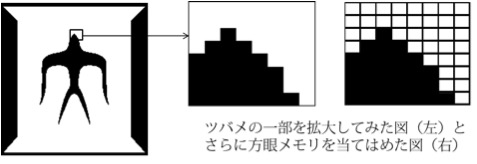
\includegraphics[scale=0.4]{./Figure/TITECH-logo.jpg}
%\end{frame}
%\begin{frame}
%\frametitle{音}
%  \begin{itemize}
%\item つぎは音データ
%\item 波の符号化
%    \begin{itemize}
%\item (a) は波形
%\item (b) は標本化
%\item (c) はそれぞれの標本値
%\item この標本値を順番にならべた二進列
%    \end{itemize}
%\item 音符の符号化 (Standard MIDI)
%    \begin{itemize}
%\item 音符やテンポを符号化
%\item \movie[once,externalviewer]{\beamerbutton{.mid}}{./Figure/Nodame.mid}
%    \end{itemize}
%  \end{itemize}
%  \begin{center}
%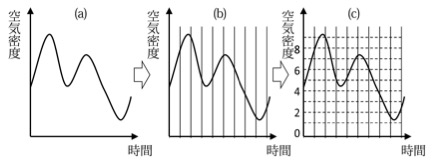
\includegraphics[scale=0.4]{./Figure/wave.jpg}
%  \end{center}
%\end{frame}
%
%%% COMPUTER
%
%\section{コンピュータの中では}
%\begin{frame}
%\frametitle{コンピュータの中では}
%  \begin{itemize}
%\item コンピュータの命令自体も符号化されてます
%\item CPU (Central Processing Unit) ごとに命令セットも符号も異なっています
%\item ここでは CPU が命令を実行するサイクルについて見てみます
%  \end{itemize}
%  \begin{center}
%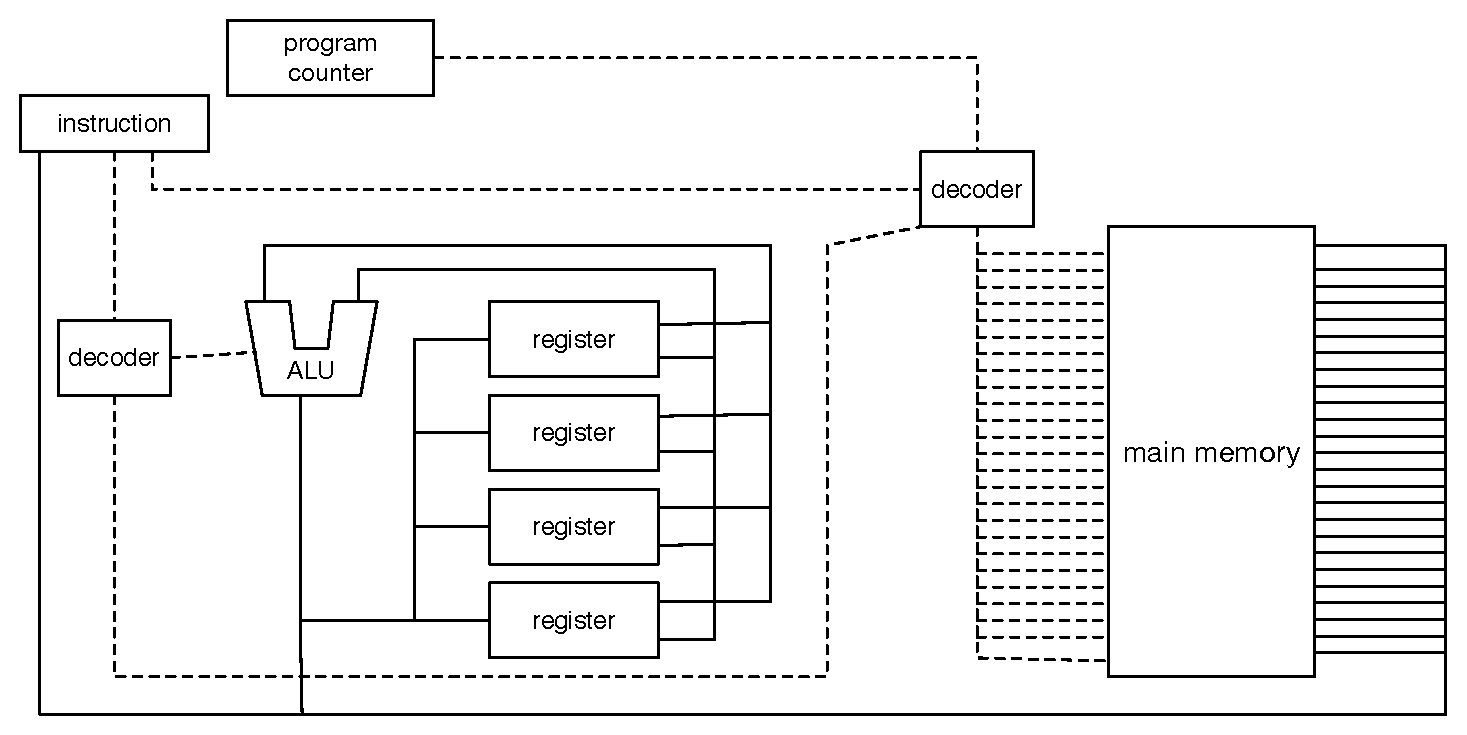
\includegraphics[scale=0.4]{./Figure/elementaryCS-figCPU}
%  \end{center}
%\end{frame}
%\begin{frame}
%\frametitle{演算のサイクル}
%  \begin{enumerate}
%\scriptsize
%\item instruction に命令をフェッチ
%\item メインメモリからレジスタにデータを移動
%\item ALU (Arithmetic and Logic Unit) がレジスタからデータを取り出す
%\item ALU で演算
%\item 結果をレジスタに書き込む
%\item レジスタからメインメモリにデータを移動
%\item ADD cx dx bx という命令を例にすると下図のようになります
%  \end{enumerate}
%  \begin{center}
%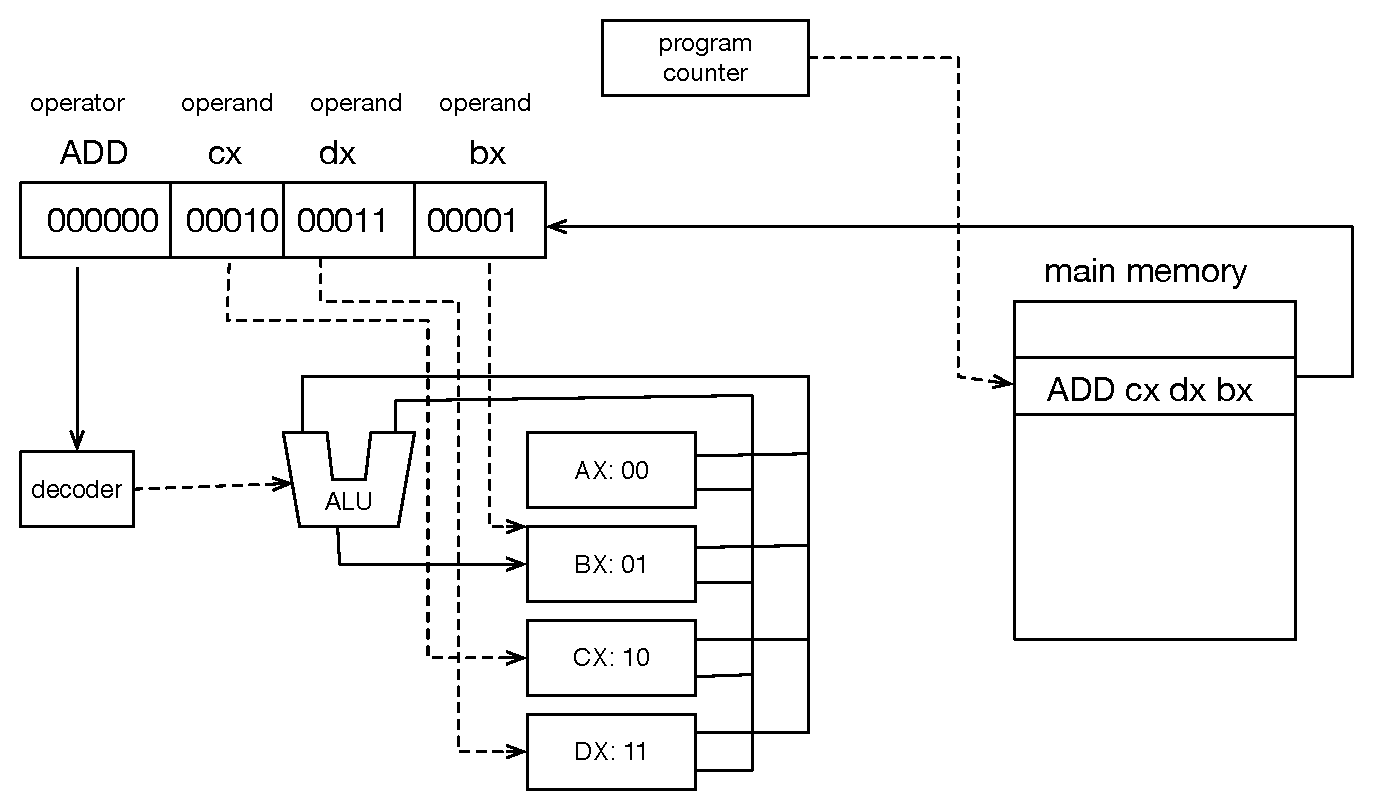
\includegraphics[scale=0.3]{./Figure/elementaryCS-figCycle}
%  \end{center}
%\end{frame}
\section{計算 = \(\pm 1\) と繰り返し}
\subsection{計算とは}
\begin{frame}
\frametitle{計算とは}
  \begin{itemize}
\item つぎは計算について
\item 計算には入力と出力があって
\item 入力と出力の関係をとくに関数とよぶ
\item この場合,ある入力に対して出力は一意に決まる
\item また関数には適当な名前をつけることができる
\item 関数を合成してより複雑な計算を実現していく
\item ここまではまだ入出力の関係としか云っていない
  \end{itemize}
  \begin{example}[最大公約数]
最大公約数 \(gcd(n,m)\) は \(n, m\) の公約数で最大ものと定義されるが,どう求めるか方法は書いていない
  \end{example}
\end{frame}
\begin{frame}[fragile,shrink]
\frametitle{計算の方法}
  \begin{itemize}
\item 計算の方法について考える
\item 計算機科学では関数といった時はこちらの意味
\item 計算の方法のことをアルゴリズム (algorithm) といっている
\item アルゴリズムとデータを特定の形式で書いたものがプログラム
  \end{itemize}
  \begin{lstlisting}[caption={最大公約数},label=gcd]
# Greatest common divisor
# Input: 自然数 x, y
# Output: gcd(x,y)
###

def gcd(x,y):
  ans=1
  n=min(x,y)
  for i in range(1,n):
    if (x%i==0) and (y%i==0):
      ans=i
  return (ans)
print(gcd(x,y))
  \end{lstlisting}
\hfill{\hyperlink{if}{\beamerbutton{Back to if-slide}}}
\end{frame}
\subsection{計算の基本要素}
\begin{frame}[fragile]
\frametitle{計算の基本要素}
\framesubtitle{計算 = \(\pm 1\) と繰り返し}
  \begin{itemize}
\item 合成していくとして最も基本となるものは何か
\item 結論から云ってしまえば,ある値に $\pm 1$ する操作と繰り返しと条件分岐である
  \end{itemize}
  \begin{lstlisting}[caption={加算},label=add]
# add.py
# Input: 自然数 a, b
# Output: a + b
###

a = int(input("? "))  # 入力された自然数を a に代入
b = int(input("? "))  # 入力された自然数を b に代入
wa = a                # a の値を wa に代入
while b > 0:          # b が 0 より大きい間は end までを繰り返す
  wa = wa + 1         #   wa + 1 の値を wa に代入
  b = b - 1           #   b - 1 の値を b に代入
print(wa)             # wa の値を出力
  \end{lstlisting}
\end{frame}
\begin{frame}[fragile,label=mult,shrink]
\frametitle{基本要素だけの乗算}
  \begin{lstlisting}[caption={乗算},label=lst:mult]
# mult_basiconly.py
# Input: 自然数 x, y
# Output: x * y
###

x = int(input("x? "))       # 入力された自然数を x に代入
y = int(input("y? "))       # 入力された自然数を y に代入
seki = 0                    # seki を 0 で初期化
while y > 0:                # y が 0 より大きい間は end までを繰り返す
  a = seki
  b = x
  wa = a                    # 和のプログラム add.py を挿入
  while b > 0:
    wa = wa + 1
    b = b - 1
  seki = wa                 # wa の値 (seki + x) を seki に代入
  y = y - 1                 # y - 1 の値を y に代入
print(seki)                 # seki の値を出力
  \end{lstlisting}
\hfill{\hyperlink{composit}{\beamerbutton{Back to composit-slide}} \hyperlink{while}{\beamerbutton{Back to while-slide}}}
\end{frame}
\section{プログラムの書き方}
\subsection{プログラミングのための仕掛け}
\begin{frame}[fragile]
\frametitle{プログラミングのための仕掛け}
  \begin{itemize}
\item プログラミング言語にはプログラミングのための 3 つの仕掛けがある
    \begin{itemize}
\item 基本式: プログラミングに関わる最も単純なもの
\item 組合せ法: 単純なものからより複雑なものをつくる (構文として定義されている)
\item 抽象化法: 合成物に名前をつけ基本式と同様に扱う
    \end{itemize}
\item データについても同様
  \end{itemize}
\end{frame}
\begin{frame}[fragile]
\frametitle{Python における基本式}
  \begin{itemize}
\item 式の基本要素は 自然数,整数,実数などがある
    \begin{itemize}
\item 自然数の例: \(286, 386, 486\) 
\item 講義では自然数だけあつかうので注意
    \end{itemize}
\item 基本要素と演算子 \(+, -, *, \slash\slash, \%, **\) などを組み合わせて式をつくる
    \begin{itemize}
\item 自然数の例: \(286+386, 486\) 
\item 入れ子にできます: \(286+(386+486)\) 
    \end{itemize}
\item 式には名前をつけることができ,この名前のことを変数と呼でいます
\item その名前で参照することもできます
    \begin{itemize}
\item 例: \(\mbox{abc}=286+386\) 
\item 例: \(\mbox{efg}=\mbox{abc}+486\) 
    \end{itemize}
\item $=$ は論理記号ではなくて代入をあらわすので注意
\item abc は \(\mbox{a}\times\mbox{b}\times\mbox{c}\) ではなく変数名なので注意
  \end{itemize}
\end{frame}
%\begin{frame}[fragile]
%\frametitle{Ruby における論理演算子}
% \begin{center}
%  \begin{tabular}{c|c|c}
%算術演算子&使用例&意味\\\hline
%+& x $+$ y & x と y の足し算\\
%-& x $-$ y & x と y の引き算\\
%*& x $*$ y & x と y のかけ算\\
%$\slash$& x $\slash$ y & x を y 割った商\\
%\%& x $\%$ y & x を y 割ったあまり\\
%**& x $**$ y & x の y 乗\\\hline
%論理演算子&使用例&意味\\\hline
%==& x == y & x と y が等しいなら真\\
%!=& x != y & x と y が等しくないなら真\\
%>=& x >= y & x は y 以上なら真\\
%<=& x <= y & x は y 以下なら真\\
%>& x > y & x は y より大きいなら真\\
%<& x < y & x は y より小さいなら真\\
%  \end{tabular}
% \end{center}
%\end{frame}
%\begin{frame}[fragile]
%\frametitle{論理の合成}
% \begin{center}
%  \begin{tabular}{c|c|c}
%論理演算子&使用例&意味\\\hline
%\&\& & p \&\& q & 論理積: 両方が真なら真\\
%$\|$ & p $\|$ q & 論理和: いずれかが真なら真\\
%! & ! p & p の否定\\
%  \end{tabular}
% \end{center}
%\end{frame}
\begin{frame}[label=composit]
\frametitle{Python における合成}
  \begin{itemize}
\item 式を順番に並べる
\item 実行は上から下へ,左から右に順番に実行される
\item 前に実行された式の結果は変数をもちいて参照
\item 実行順序を変えたいときは while や if を使う
\item \hyperlink{mult}{\beamerbutton{Jump to an example}}
  \end{itemize}
\end{frame}
\begin{frame}[fragile,label=if]
\frametitle{if 文}
  \begin{itemize}
\item 条件によって実行順序を変更する
\item \hyperlink{gcd}{\beamerbutton{Jump to an example}}
\item 条件式は \href{https://docs.python.org/ja/3/reference/expressions.html#comparisons}{\beamerbutton{Python ドキュメント 6.10, 6.11, 6.12 節}}参照
  \end{itemize}
\end{frame}
\begin{frame}[fragile,label=while]
\frametitle{while 文}
  \begin{itemize}
\item 実行列を繰り返し実行する
\item \hyperlink{mult}{\beamerbutton{Jump to an example}}
  \end{itemize}
\end{frame}
%%%
% Homework 1
%%%
\subsection{宿題 1 を動かしてみる}
\begin{frame}[fragile,shrink]
\frametitle{宿題 1 を動かしてみる}
\framesubtitle{宿題 1 \textendash $\pm 1$だけで四則演算を作る}
  \begin{itemize}
\item \href{https://sites.google.com/a/presystems.xyz/sample/home/elementary-computer-science}{\beamerbutton{https://sites.google.com/a/presystems.xyz/sample/home/elementary-computer-science}} に div-skeleton.py と sub-skeleton.py があるはずなのでそれを完成させて実行する
\item OCW-i から提出
\item ファイル名に日本語文字は使用しないでください
  \end{itemize}
  \begin{columns}
    \begin{column}{0.45\textwidth}
      \begin{lstlisting}[caption={sub.py},label=lst:sub]
# sub.py
# Input: 自然数 a, b
# Output: a - b

a = int(input("a? "))
b = int(input("b? "))
sa = a               
while    :
  sa = 
  b = 
print(sa)
      \end{lstlisting}
    \end{column}
    \begin{column}{0.45\textwidth}
      \begin{lstlisting}[caption={div.py},label=lst:div]
# div.py
# Input: 自然数 x, y
# Output: x ÷ y の商と余り

x = int(input("x? "))
y = int(input("y? "))
shou = 
amari = 
while    :
  shou = 
  amari = amari - y
print(shou)
print(amari)
      \end{lstlisting}
    \end{column}
  \end{columns}
\end{frame}
%
%%% PROGRAMMING ENVIRONMENT
%
\section{開発環境構築}
\subsection{Python3 環境構築}
\begin{frame}[shrink]
\frametitle{環境構築}
\framesubtitle{Python3}
  \begin{itemize}
\item Python を利用するためには各自の PC 上に環境を構築する必要があります
\item すでに python 開発環境を持っている人は以下の作業は不要です
\item 各状況に合わせて環境を作っていきます
    \begin{itemize}
\item Cloud で利用したい方は\href{https://www.pythonanywhere.com/}{\beamerbutton{https://www.pythonanywhere.com/}}で beginner account を作成(無料でインストール不要です)
\item Windows, Mac OSX, Linux で自分の PC に環境を作りたい方は\href{https://www.python.jp/install/install.html}{\beamerbutton{https://www.python.jp/}}を参照
    \end{itemize}
  \end{itemize}
\end{frame}
\begin{frame}[shrink,containsverbatim]
\frametitle{Pythonanywhere のアカウント開設}
  \begin{itemize}
\item ``Start running Python on line in less than a minute'' をクリック
  \end{itemize}
\includegraphics[width=1\textwidth]{../InformationLiteracy/Figure/IL-figStartAnywhere.jpg}
\end{frame}
\begin{frame}[shrink,containsverbatim]
\frametitle{Pythonanywhere のアカウント作成}
  \begin{itemize}
\item ``Create a Biginner account'' をクリック
\item 無料のアカウントを作成します
  \end{itemize}
\includegraphics[width=1\textwidth]{../InformationLiteracy/Figure/IL-figCreateAnywhereAccount.jpg}
\end{frame}
\begin{frame}[shrink,containsverbatim]
\frametitle{Pythonanywhere のアカウント登録}
  \begin{itemize}
\item ``Username'' を入力(任意)
\item ``Email'' を入力(m ドメイン以外でもかまいません)
\item ``Password'' を入力
\item ``I agree$\ldots$'' にチェック
\item ``Register'' をクリック
  \end{itemize}
\includegraphics[width=1\textwidth]{../InformationLiteracy/Figure/IL-figAnywhereRegister.jpg}
\end{frame}
\begin{frame}[shrink,containsverbatim]
\frametitle{登録後の画面}
  \begin{itemize}
\item 登録アドレスにメイルが届くので確認
\item 以下のような画面が見えれば OK
  \end{itemize}
  \begin{itembox}{登録後の画面}
\includegraphics[width=1\textwidth]{../InformationLiteracy/Figure/IL-figAnywhereDashboard.jpg}
  \end{itembox}
\end{frame}
\begin{frame}[shrink,containsverbatim]
\frametitle{自身の PC 上にインストールひと}
  \begin{itemize}
\item Idle を起動してください
  \end{itemize}
  \begin{columns}[t]
    \begin{column}{0.5\textwidth}
      \begin{itembox}{\footnotesize Mac, Linux のひと}
        \begin{itemize}
\scriptsize
\item ターミナルを起動して idle3 と入力
        \end{itemize}
        \begin{verbatim}
> idle3
        \end{verbatim}
      \end{itembox}
    \end{column}
    \begin{column}{0.5\textwidth}
      \begin{itembox}{\footnotesize Windows のひと}
        \begin{itemize}
\item スタートメニューから IDLE を起動
        \end{itemize}
      \end{itembox}
    \end{column}
  \end{columns}
\end{frame}
\begin{frame}[shrink,containsverbatim]
\frametitle{開発統合環境}
\framesubtitle{IDLE と Pythonanywhere}
  \begin{itemize}
\item Mac, Windows, Linux の人もこれで準備ができました
\item それぞれ以下のような画面が見えるはずです
\item 以後,いずれかの開発統合環境を利用していきます
\item Pythonanywhere や IDLE は編集,実行が統合された環境を提供しています
\item IDLE の使い方は\href{https://docs.python.org/ja/3/library/idle.html?highlight=idle}{\beamerbutton{Python 公式}}を参照
    \begin{itemize}
\item \href{http://www.isc.meiji.ac.jp/~mizutani/python/intro1_python.html}{\beamerbutton{http://www.isc.meiji.ac.jp/~mizutani/python/intro1\_python.html}}も参考になるかも
    \end{itemize}
  \end{itemize}
  \begin{columns}[c]
    \begin{column}{5cm}
\includegraphics[width=1\textwidth]{../InformationLiteracy/Figure/IL-figIDLE.jpg}
    \end{column}
    \begin{column}{5cm}
\includegraphics[width=1\textwidth]{../InformationLiteracy/Figure/IL-figPythonanywhere.jpg}
    \end{column}
  \end{columns}
\end{frame}
\subsection{動作確認}
\begin{frame}[shrink,containsverbatim]
\frametitle{開発環境テスト用コード}
%\vspace{-2zw}
%  \begin{lstlisting}[caption={環境テスト用コード},label=lst:test,numbers=none]
%import matplotlib.pyplot as plt
%print('Hello World')
%plt.plot([1, 2, 3, 4])
%plt.show()
%  \end{lstlisting}
  \begin{itemize}
\item \href{https://sites.google.com/presystems.xyz/elementarycs/top}{\beamerbutton{https://sites.google.com/presystems.xyz/elementarycs/top}} 
からhello.pyをダウンロード
  \end{itemize}
\vspace{-1em}
  \begin{columns}[t]
    \begin{column}{0.5\textwidth}
      \begin{itembox}{\footnotesize IDLE 利用のひと}
        \begin{itemize}
\scriptsize
\item File->Open で hello.py を開く
        \end{itemize}
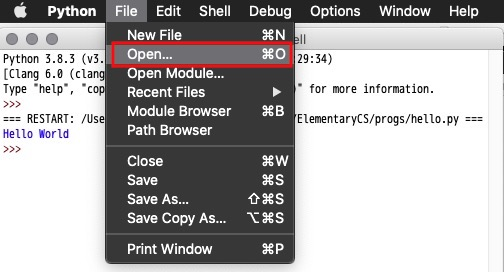
\includegraphics[width=1\textwidth]{./Figure/elementaryCS-figOpenFile.jpg}
      \end{itembox}
    \end{column}
    \begin{column}{0.5\textwidth}
      \begin{itembox}{\footnotesize Pythonanywhere 利用のひと}
\scriptsize
        \begin{itemize}
\item 右上 ``Files'' をクリック
\item ''upload'' をクリックして hello.py をアップロード
\item hello.py をクリックすると中が見れます
        \end{itemize}
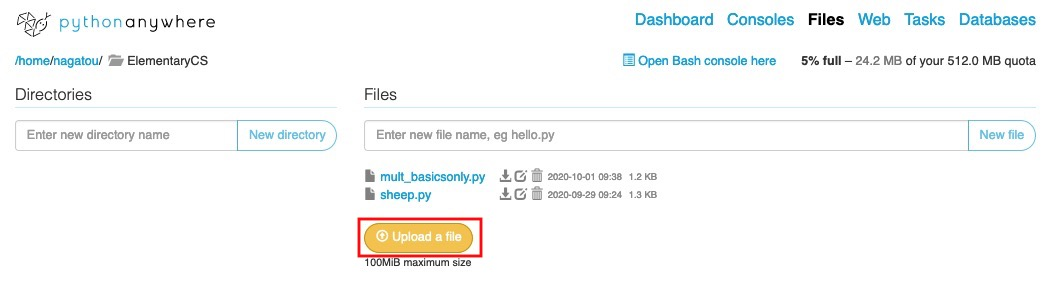
\includegraphics[width=1\textwidth]{./Figure/elementaryCS-figUpload.jpg}
      \end{itembox}
    \end{column}
  \end{columns}
\end{frame}
\begin{frame}[shrink,containsverbatim]
\frametitle{プログラムの実行}
%  \begin{itemize}
%\item \href{https://sites.google.com/a/presystems.xyz/sample/home/information-literacy}{\beamerbutton{https://sites.google.com/a/presystems.xyz/sample/home/information-literacy}}から test.py をダウンロード
%  \end{itemize}
  \begin{columns}[t]
    \begin{column}{0.5\textwidth}
      \begin{itembox}{\footnotesize IDLE 利用のひと}
        \begin{itemize}
\scriptsize
\item Run->Run Module をクリック
\item ``Hello World'' が表示されれば正常
        \end{itemize}
\includegraphics[width=1\textwidth]{../InformationLiteracy/Figure/IL-figTestIDLE.jpg}
      \end{itembox}
    \end{column}
    \begin{column}{0.5\textwidth}
      \begin{itembox}{\footnotesize Pythonanywhere 利用のひと}
\scriptsize
        \begin{itemize}
\item Run this file をクリック
\item 下半分の黒い画面に ``Hello World'' と表示されれば正常
\item 下半分の黒い画面で exit() と入力してください
        \end{itemize}
\includegraphics[width=1\textwidth]{../InformationLiteracy/Figure/IL-figTestCloud.jpg}
      \end{itembox}
    \end{column}
  \end{columns}
\end{frame}


%
%%% QUIZ 1
%
\part{CS 第 1\textemdash 課題 1}
\frame{
  \frametitle{CS 第 1 \textemdash 課題 1}
\scriptsize
  \tableofcontents[part=3]
}
%
%%% QUIZ 1
%
\section{課題 1 演習ガイド}
\subsection{課題 1 の説明}
\begin{frame}
\frametitle{課題 1の説明}
\framesubtitle{四則演算でアニメーション}
  \begin{itemize}
\item 課題: 四則演算でアニメーションを作成してください
    \begin{itemize}
\item 動きがあること
\item 計算だけで動かすこと
    \end{itemize}
\item 提出物:
    \begin{itemize}
\item 作成したアニメーションプログラムのソースコード (anime.py)
\item 作成したアニメーションプログラムの使い方の説明
\item 作成したアニメーションプログラムの計算の仕組みの説明
      \begin{itemize}
\item 工夫した点も書くこと
      \end{itemize}
    \end{itemize}
\item 採点者はソースコードを読まないと仮定して説明すること
\item Python 言語の説明は不要
\item 期限は来週のこの時間まで
  \end{itemize}
\end{frame}
%\begin{frame}[fragile]
%\frametitle{四則演算でアニメーションの例}
%  \begin{itemize}
%\item 10 個の自然数
%\item 先頭は 1 にしないとずれる
%  \end{itemize}
%\tiny
%  \begin{columns}
%    \begin{column}{0.55\textwidth}
%      \begin{lstlisting}[caption={smile.py},label=smile-data]
%# smile.py
%# 入力: 10個の自然数
%# 出力: スマイルマーク
%
%d1 =1000000000000000000000000000
%d2 =1000000000110000110000000000
%d3 =1000000000110000110000000000
%d4 =1000000000000000000000000000
%d5 =1000001100000000000011000000
%d6 =1000000110000000000110000000
%d7 =1000000011000000001100000000
%d8 =1000000000111111110000000000
%d9 =1000000000000000000000000000
%d10=1000000000000000000000000000
%      \end{lstlisting}
%    \end{column}
%    \begin{column}{0.4\textwidth}
%      \begin{lstlisting}[caption={smile.py},label=smile-body,firstnumber=last]
%t = 0
%while t < 15
%  puts(t)
%  puts(d1)
%  puts(d2)
%  puts(d3)
%  puts(d4)
%  puts(d5)
%  puts(d6)
%  puts(d7)
%  puts(d8)
%  puts(d9)
%  puts(d10)
%  puts()   # 空行を出力
%  sleep(1) # 1秒休む
%  t = t + 1
%end
%      \end{lstlisting}
%    \end{column}
%  \end{columns}
%\end{frame}
%\begin{frame}[fragile]
%\frametitle{スマイルを動かしてみる}
%\scriptsize
%  \begin{itemize}
%\item ここでいう動かすとはデータを計算で変化させていってそれを描画
%\item 10 で割っているので一番右のけたが落ちていきます
%  \end{itemize}
%  \begin{lstlisting}[caption={smile2.py},label=smile-destroy]
%# smile2.py
%# 入力: 10個の自然数
%# 出力: スマイルマークが,どうなるか?
%...
%while t < 29
%...
%  d1 = d1 / 10
%  d2 = d2 / 10
%  d3 = d3 / 10
%  d4 = d4 / 10
%  d5 = d5 / 10
%  d6 = d6 / 10
%  d7 = d7 / 10
%  d8 = d8 / 10
%  d9 = d9 / 10
%  d10 = d10 / 10
%
%  t = t + 1
%end
%  \end{lstlisting}
%\end{frame}
\begin{frame}[fragile,shrink]
\frametitle{ひつじさんを動かしてみる}
  \begin{itemize}
\scriptsize
\item 大きな数字を定義して
\item 各桁をひとつの画素とみなす
\item 各桁は 0\textendash 9 でこの違いで絵にする
\item 14 個の自然数
\item 先頭は 1 にしないとずれる
\item 動かすときは桁をシフトさせて (ここでは 10 で割っている) 動かす
  \end{itemize}
  \begin{lstlisting}[caption={sheep.py (declaration)},label=sheep-data]
################
# pattern def. #
################
d0  = 1000000000000000000000000000000000000000000000000000000000
d1  = 1000000000000000000000000011111111000000000000000000000000
d2  = 1000000000000000000000001110000000110000000000000000000000
d3  = 1000000011111111111110011000011000111111000000000000000000
d4  = 1000001110000000000000001100111000110000110000000000000000
d5  = 1000001100000000000000000111110011000100011000000000000000
d6  = 1000001100000000000000000000000000000001111000000000000000
d7  = 1000001100000000000000000000000000000111000000000000000000
d8  = 1000001100000000000000000000000000011100000000000000000000
d9  = 1000001100000000000000000000000000011000000000000000000000
d10 = 1000001100000000000000000000000000111000000000000000000000
d11 = 1000000011000110001111111000110001110000000000000000000000
d12 = 1000000000111001110000000111001110000000000000000000000000
d13 = 1000000000000000000000000000000000000000000000000000000000
  \end{lstlisting}
\end{frame}
\begin{frame}[fragile,shrink]
\frametitle{ひつじさんを動かしてみる}
  \begin{itemize}
\scriptsize
\item 動かすときは桁をシフトさせて (ここでは 10 で割っている) 動かす
\item {\tt a0} を足しているのは絵がずれないようにするため
  \end{itemize}
  \begin{lstlisting}[caption={sheep.py (shift)},label=sheep-shift,firstnumber=last]
      # shift #
      a0 = d0

      a1  = (a1 -  a0) // 10 + a0
      a2  = (a2  - a0) // 10 + a0
      a3  = (a3  - a0) // 10 + a0
      a4  = (a4  - a0) // 10 + a0
      a5  = (a5  - a0) // 10 + a0
      a6  = (a6  - a0) // 10 + a0
      a7  = (a7  - a0) // 10 + a0
      a8  = (a8  - a0) // 10 + a0
      a9  = (a9  - a0) // 10 + a0
      a10 = (a10 - a0) // 10 + a0
      a11 = (a11 - a0) // 10 + a0
      a12 = (a12 - a0) // 10 + a0
      a13 = (a13 - a0) // 10 + a0
      a14 = (a14 - a0) // 10 + a0
      a15 = (a15 - a0) // 10 + a0
      a16 = (a16 - a0) // 10 + a0
      a17 = (a17 - a0) // 10 + a0
      a18 = (a18 - a0) // 10 + a0
      a19 = (a19 - a0) // 10 + a0
      a20 = (a20 - a0) // 10 + a0
  \end{lstlisting}
\end{frame}


%% ARRAY

\part{配列}
\frame{
  \frametitle{配列}
\scriptsize
  \tableofcontents[part=4]
}
\section{課題 2 演習ガイド}
%
%%% TERMINAL
%
\subsection{配列}
\begin{frame}[containsverbatim]
\frametitle{配列}
  \begin{itemize}
\item いくつかのデータオブジェクトを1つにまとめて扱い時がある
\item 配列は,データブジクトの順序づけられた集まり
\item 配列の各オブジェクトを配列の要素と呼びます
\item 各要素は 0 から始まる自然数に対応付けられていて
\item 自然数のことをインデックスと呼んでいます
\item 各要素は配列名[インデックス]で参照することができます
  \end{itemize}
\tiny
  \begin{columns}
    \begin{column}{0.45\textwidth}
      \begin{lstlisting}[caption={単純な変数},label=naive]
d1 =  1000000000000000000000000000
d2 =  1000000000110000110000000000
d3 =  1000000000110000110000000000
d4 =  1000000000000000000000000000
d5 =  1000001100000000000011000000
d6 =  1000000110000000000110000000
d7 =  1000000011000000001100000000
d8 =  1000000000111111110000000000
d9 =  1000000000000000000000000000
      \end{lstlisting}
    \end{column}
    \begin{column}{0.45\textwidth}
      \begin{lstlisting}[caption={配列},label=array]
 d = [1000000000000000000000000000,
      1000000000110000110000000000,
      1000000000110000110000000000,
      1000000000000000000000000000,
      1000001100000000000011000000,
      1000000110000000000110000000,
      1000000011000000001100000000,
      1000000000111111110000000000,
      1000000000000000000000000000]
      \end{lstlisting}
    \end{column}
  \end{columns}
\end{frame}
\begin{frame}[containsverbatim]
\frametitle{配列の参照と代入}
  \begin{itemize}
\item 連続したメモリ領域を確保
\item 先頭を 0 としてインデックスで参照 (ここは板書します)
  \end{itemize}
\tiny
  \begin{columns}
    \begin{column}{0.5\textwidth}
      \begin{lstlisting}[caption={代入},label=array-assign]
 d = [0]*9
 d[0]=1000000000000000000000000000
 d[1]=1000000000110000110000000000
 d[2]=1000000000110000110000000000
 d[3]=1000000000000000000000000000
 d[4]=1000001100000000000011000000
 d[5]=1000000110000000000110000000
 d[6]=1000000011000000001100000000
 d[7]=1000000000111111110000000000
 d[8]=1000000000000000000000000000
      \end{lstlisting}
    \end{column}
    \begin{column}{0.35\textwidth}
      \begin{lstlisting}[caption={参照},label=array-ref]
 for i in range(9):
   print(d[i])
      \end{lstlisting}
\centering
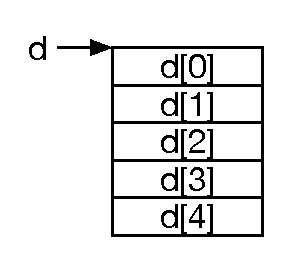
\includegraphics[scale=0.5]{./Figure/elementaryCS-figArray.eps}
    \end{column}
  \end{columns}
\end{frame}
\begin{frame}[containsverbatim]
\frametitle{配列の例}
  \begin{itemize}
\item 総和を求める
\item \lstref{lst:sum6}: 整数の配列を宣言する例
\item \lstref{lst:sum}: 入力した整数を配列にする例
  \end{itemize}
  \begin{columns}
    \begin{column}{0.35\textwidth}
      \begin{lstlisting}[caption={sum6.py},label=lst:sum6]
a=[2,4,6,8,10,12]
s=0
for k in range(len(a)):
  s=s+a[k]
  k=k+1
print(s)
      \end{lstlisting}
    \end{column}
    \begin{column}{0.6\textwidth}
      \begin{lstlisting}[caption=sum.py,label=lst:sum]
a = list(map(int,input("numbers? ").split()))
s=0
for k in range(len(a)):
  s=s+a[k]
  k=k+1
print(s)
      \end{lstlisting}
    \end{column}
  \end{columns}
\end{frame}
\begin{frame}[containsverbatim, shrink]
\frametitle{最大値を求める}
\framesubtitle{宿題 2}
  \begin{itemize}
\item \href{https://sites.google.com/presystems.xyz/elementarycs/top}{\beamerbutton{https://sites.google.com/presystems.xyz/elementarycs/top}} の max-skeleton.py を完成させる
\item 最大値=max\((a_1, a_2,\cdots,a_n)\)
\item {\tt for j in range(0,n)} は {\tt j} を 0 から n-1 まで繰り返すという意味
  \end{itemize}
\vspace{-1em}
  \begin{columns}
    \begin{column}{0.6\textwidth}
      \begin{lstlisting}[caption={max.py},label=lst:max]
# max.py
# 入力: 整数の列
# 出力: 最大値
array = list(map(int,input("numbers? ").split()))
if not array:  # array が空の場合
    raise ValueError("...")  # 入力エラー
# 以下が計算部分
max_value = array[0]      # array[0] を一時的に最大値に
max_index = 0
for i in range(0,(len(array))):
  if :                    # より大きな数を探す
    max_value =
    max_index =
print(max_value, max_index)
      \end{lstlisting}
    \end{column}
    \begin{column}{0.35\textwidth}
      \begin{itembox}{出力例}
\scriptsize
> python3 max.py\\
numbers? -3 8 19 -4\\
19 2
      \end{itembox}
    \end{column}
  \end{columns}
\end{frame}
%
%%% STRINGS
%
\subsection{文字列}
\begin{frame}
\frametitle{文字データの表現}
  \begin{itemize}
\item コンピュータは数値だけでなく文字も処理することができる
\item 文字はコード化されて処理される
\item 文字列は文字の配列
  \end{itemize}
\end{frame}
\begin{frame}
\frametitle{文字コード}
  \begin{itemize}
\item コードとは,文字や記号をコンピュータで扱うための符号です
\item コンピュータ内では適当な正整数が文字や記号に割り振られています
    \begin{itemize}
\item 整数は 2 進数で表されているので 0 と 1 の列にコード化されます
    \end{itemize}
\item コードは任意に決めることもできます
\item しかし,各コンピュータで違っていては不都合が生じます
\item 異なるコンピュータでは全く違った文字になってしまうかも知れません
    \begin{itemize}
\item 文字コードが違っているとうまく表示できません
    \end{itemize}
  \end{itemize}
\end{frame}
\begin{frame}
\frametitle{コードの違いの例}
  \begin{itemize}
\item 3 という文字のコードの例です
\item 下の図は電光掲示板の例です
\item 左の図では 110 1110$_{(2)}$ とコードを割り当てています
\item 右の図では 111 1100$_{(2)}$ とコードを割り当てています
\item このように違ったコードを対応づけることもできます
  \end{itemize}
  \begin{example}[電光掲示板の例]
    \begin{center}
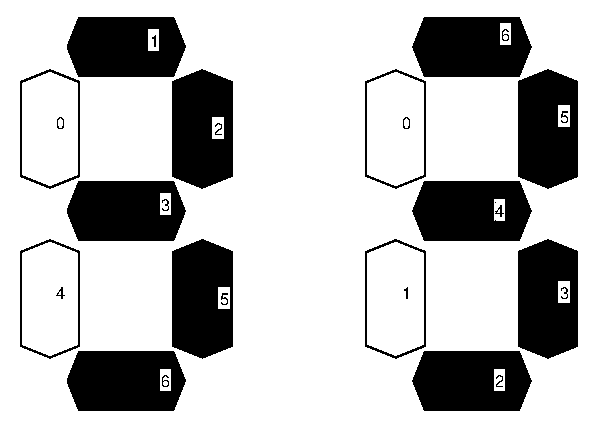
\includegraphics[scale=0.5]{./Figure/ComputerLiteracy-figThree.eps}
    \end{center}
  \end{example}
\end{frame}
\begin{frame}
\frametitle{ASCII コード}
  \begin{itemize}
\item 共通のコード体系として ASCII コードが策定されました
\item これは英語のアルファベットと数字と記号にコードを割り当てています
    \begin{itemize}
\item \href{https://en.wikipedia.org/wiki/ASCII\#/media/File:US-ASCII\_code\_chart.png}{\beamerbutton{ASCII Code Chart}}
    \end{itemize}
  \end{itemize}
\end{frame}
\begin{frame}
\frametitle{日本語漢字のコード体系}
  \begin{itemize}
\item 現在は日本語など漢字圏の文字もコードが割り当てられています
\item JIS, Shift-JIS, EUC, Unicode があります
    \begin{itemize}
\item これらは異なるコード体系です
\item 同じ文字でも異なるコードが割り当てられています
    \end{itemize}
\item 漢字圏で Unicode 以前に用いていたコードの規格
    \begin{itemize}
\item 日本: JIS X 0208-1990, JIS X 0212-1990(第一水準,第二水準,補助漢字)
\item 中国: GB 2312-80, GB 12345-90$\cdots$
\item 台湾: CNS 111643-1986
\item 韓国: KS C 5601-1987, KS C 5657-1991
    \end{itemize}
\item Python3 は Unicode を利用しています
  \end{itemize}
\end{frame}
\begin{frame}[containsverbatim, shrink]
\frametitle{Python での文字列}
  \begin{itemize}
\item 文字列は各文字の配列として扱える
\item {\texttt str} という名前の配列の各要素に一文字入っている
\item 0 番目から順番にインデックスで参照できる
  \end{itemize}
  \begin{columns}
    \begin{column}{0.55\textwidth}
      \begin{lstlisting}[caption={stringPrint.py},label=lst:strprt]
# stringPrint.py
# 文字列処理の練習プログラム
# 入力: 文字列
# 出力: 文字列の文字を1行1文字で出す
import os

os.system('clear')
str = (input("strings? ")).encode("ascii")
print(str)
for k in range(0,len(str)):
   print(chr(str[k]), hex(str[k]))
      \end{lstlisting}
    \end{column}
    \begin{column}{0.35\textwidth}
      \begin{itembox}{出力例}
\scriptsize
> python3 stringPrint.py\\
strings? Ice\%cream\\
I 0x49\\
c 0x63\\
e 0x65\\
\% 0x25\\
c 0x63\\
r 0x72\\
e 0x65\\
a 0x61\\
m 0x6d
      \end{itembox}
    \end{column}
  \end{columns}
\end{frame}
\begin{frame}[containsverbatim]
\frametitle{文字列の表現}
  \begin{itemize}
\item 文字列は文字の配列
\item 各文字はその符号(文字コード)で表されて
\item 各要素に各文字コードを格納
  \end{itemize}
  \begin{columns}
    \begin{column}{0.4\textwidth}
      \begin{itembox}{出力例}
\scriptsize
> python3 stringPrint.py\\
strings? Ice\%cream\\
I 0x49\\
c 0x63\\
e 0x65\\
\% 0x25\\
c 0x63\\
r 0x72\\
e 0x65\\
a 0x61\\
m 0x6d
      \end{itembox}
    \end{column}
    \begin{column}{0.6\textwidth}
      \begin{center}
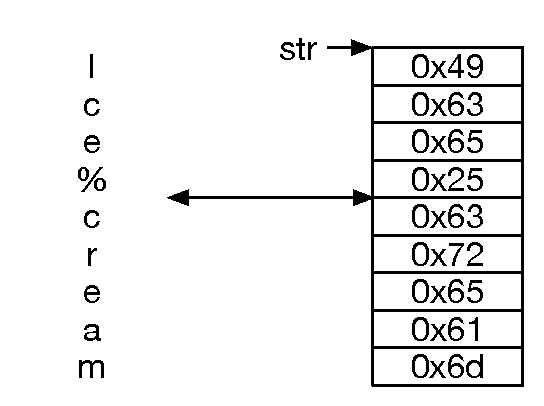
\includegraphics[scale=0.5]{./Figure/elementaryCS-figStrings.eps}
      \end{center}
    \end{column}
  \end{columns}
\end{frame}
\begin{frame}[containsverbatim, shrink]
\frametitle{英小文字だけを画面に出力}
\framesubtitle{宿題 3}
  \begin{itemize}
\item \href{https://sites.google.com/presystems.xyz/elementarycs/top}{\beamerbutton{https://sites.google.com/presystems.xyz/elementarycs/top}} の abcPrint-skeleton.py を完成させる
  \end{itemize}
  \begin{columns}
    \begin{column}{0.6\textwidth}
      \begin{lstlisting}[caption={abcPrint.py},label=lst:lowerletterprt]
# abcPrint.py
# 文字列処理の練習プログラム,小文字だけ出力
# 入力: 文字列
# 出力: 文字列の文字で小文字のみ出力する
ss = (input("strings? ")).encode("ascii")
for k, code in enumerate(ss):
  if :                   # 小文字ならば
     print(chr(ss[k]))   # 文字を表示する
      \end{lstlisting}
    \end{column}
    \begin{column}{0.35\textwidth}
      \begin{itembox}{出力例}
\scriptsize
> python3 abcPrint.py\\
strings? Ice\%cream\\
c\\
e\\
c\\
r\\
e\\
a\\
m
      \end{itembox}
    \end{column}
  \end{columns}
\end{frame}
%
%%% QUIZ 2
%
\subsection{課題 2 予告}
\begin{frame}
\frametitle{課題 2 予告}
  \begin{itemize}
\item 来週の予定です
\item \hyperlink{quiz2}{\beamerbutton{Jump to Quiz 2}}
  \end{itemize}
\end{frame}

%
%%% SPECIAL QUIZ
%
\section{課題 S 演習ガイド}
\subsection{課題 S}
\begin{frame}[containsverbatim, shrink, label=quizS]
\frametitle{課題 S}
  \begin{itemize}
\item 自然数上の演算を整数に拡張
\item \href{https://sites.google.com/presystems.xyz/elementarycs/top}{\beamerbutton{https://sites.google.com/presystems.xyz/elementarycs/top}} からまずは integers-skeleton.py をダウンロード
\item お話していない部分も含まれるので調べながらやってみてください
\item ソースコード中のコメントを参照して (1)-(4) が虫食いになっているので完成させる
\item 提出は出来たところまででいいです
\item 出来なかったところはコメントにしてください
  \end{itemize}
\end{frame}

%
%%% QUIZ 2
%
\part{CS 第 1\textemdash 課題 2}
\frame{
  \frametitle{CS 第 1 \textemdash 課題 2}
\scriptsize
  \tableofcontents[part=5]
}
%
%%% QUIZ 2
%
\section{課題 2 演習ガイド}
\subsection{課題 2}
\begin{frame}[label=quiz2]
\frametitle{課題 2 テーマ}
  \begin{itemize}
\item 前回までにみたように配列は複数のデータを統一的に扱う方法を提供した
\item それ以外の例もこの課題で見ていくことにします
  \end{itemize}
  \begin{block}{やってほしいこと}
    \begin{itemize}
\item 今,自然数の組で表わされている有理数を小数表記に変換するプログラムを作ろうとしているとします
\item 配列を使って循環小数になっても停止するようにプログラム junkan.py を改良してください
\item ただし,分子は 1 に固定する
    \end{itemize}
  \end{block}
\end{frame}
\begin{frame}[containsverbatim, shrink]
\frametitle{junkan.py}
  \begin{itemize}
\item まずは junkan.py を実行してみてください
\item あまりは 0 から d-1 の有限の範囲なので,10 倍して割るを繰り返しているとどこかで同じあまりが出てくるはず
  \end{itemize}
  \begin{lstlisting}[caption={junkan.py},label=lst:rational]
# junkan.py
# 配列の使い方の練習(循環小数を循環するまで求める)
# 入力: d
# 出力: 1/d の各桁を循環するまで求める
d = int(input("1/d d(>=2)? "))
print("1/",d," を求めます")
x = 1
print("0.", end=""),
while (True):
  x = x * 10
  q = x // d
  x = x % d
  print(q, end="")
  if x == 0:
    break
print("")
  \end{lstlisting}
\end{frame}

%%
%%%% SUBROUTINE and FUNCTION
%%
\part{関数とサブルーチン}
\frame{
  \frametitle{関数とサブルーチン}
\scriptsize
  \tableofcontents[part=6]
}
%
%%% QUIZ 3
%
%\section{課題 3 演習ガイド}
%\subsection{課題 3 ガイド}
%\begin{frame}
%\frametitle{課題 3 ガイド}
%  \begin{itemize}
%\item \hyperlink{situation}{\beamerbutton{課題 3 予告}}
%\item これを通して関数,メソッド,サブルーチンの概念を見ていく
%  \end{itemize}
%\end{frame}
%
%%% FUNCTION
%
\section{関数,メソッド,サブルーチン}
\subsection{関数宣言}
\begin{frame}[containsverbatim,label=function,shrink]
\frametitle{関数,メソッド,サブルーチン}
  \begin{itemize}
\item 抽象化の方法について触れてきた
    \begin{itemize}
\item 変数: 計算の結果に名前をつけるということ
\item 配列: データの集まりを名前をつけて抽象化
    \end{itemize}
\item 今回は計算を合成する抽象化について見てみます
\item 合成したものに名前をつけて単一の手続きとして抽象化する方法
  \end{itemize}
\end{frame}
\begin{frame}[fragile,shrink]
\frametitle{Python における合成手続き}
  \begin{itemize}
\item Python では {\texttt def} というキーワードをつかって定義します
\item {\texttt def} のあとに関数名と仮引数を書いて,最後にコロン {\texttt :}(忘れずに)
\item 仮引数は関数を呼び出したときに実引数にバインドされる
\item 引数はその関数内だけで有効
  \end{itemize}
  \begin{columns}[t]
    \begin{column}{0.35\textwidth}
      \begin{lstlisting}[caption={add.py},label=lst:definefun]
a = int(input("a? "))
b = int(input("b? "))
wa = a
while b > 0:
  wa = wa + 1
  b = b - 1
print(wa)
      \end{lstlisting}
    \end{column}
    \begin{column}{0.3\textwidth}
      \begin{lstlisting}[caption={関数定義},label=lst:definefun2]
def add(x,y):
  wa = x 
  while y > 0:
    wa = wa + 1
    y = y - 1
  return(wa)
      \end{lstlisting}
    \end{column}
    \begin{column}{0.3\textwidth}
      \begin{lstlisting}[caption={関数適用},label=lst:definefun3,firstnumber=last]
def mult(x,y):
  seki = 0
  while y > 0:
    b = x
    seki = add(seki,b)
    y = y - 1
  return(seki)
      \end{lstlisting}
    \end{column}
  \end{columns}
\end{frame}
\subsection{計算の抽象化}
\begin{frame}[containsverbatim,shrink]
\frametitle{ブラックボックス抽象としての関数}
  \begin{itemize}
\item ``プログラムを部分に分ける''
\item どう分けるかが重要になる
\item 他のプログラムの部品として使え,まとまった仕事ができるようにわける
\item 部品としての関数はどう計算するかには関心をもたず,計算結果にだけ関心を持てば良い
  \end{itemize}
  \begin{columns}[t]
    \begin{column}{0.45\textwidth}
      \begin{lstlisting}[caption={集合演算},label=lst:fun_abst]
### Set operations
def union(seta,setb,result):
  global Size
  for i in range(Size):
    result[i]=seta[i] or setb[i]
def intersection(seta,setb,result):
  global Size
  for i in range(Size):
    result[i]=seta[i] and setb[i]
      \end{lstlisting}
    \end{column}
    \begin{column}{0.45\textwidth}
      \begin{lstlisting}[caption={集合演算},label=lst:fun_abst2,firstnumber=last]
def complement(seta,result):
  global Size
  for i in range(Size):
    result[i]= not seta[i]
def difference(seta,setb,result):
  global Size
  tmp=[-1]*Size
  for i in range(Size):
    complement(setb,tmp)
    intersection(seta,tmp,result)
      \end{lstlisting}
    \end{column}
  \end{columns}
\end{frame}
\begin{frame}[fragile]
\frametitle{仮引数と実引数}
  \begin{itemize}
\item 関数は仮引数というものをもつ
\item 複数の関数が同じ名前の仮引数を持っていても良い
\item 仮引数は関数の本体で有効である
\item 関数を呼び出したときの値に束縛 (bind) されて,関数の本体では呼び出し時の値に置き換えられる
\item 呼び出し時の値を実引数という
\item 一般に変数は有効範囲 (scope) が決まっている
\item 仮引数は関数本体が有効範囲である
  \end{itemize}
\end{frame}
%
%%% CRYPTOGRAPHY
%
\section{関数を使って世の中の事象を抽象化}
\subsection{暗号方式のおはなし}
\begin{frame}[fragile]
\frametitle{暗号通信}
  \begin{itemize}
\item 暗号システムを例に関数としての抽象化を見ていきます
  \end{itemize}
  \begin{center}
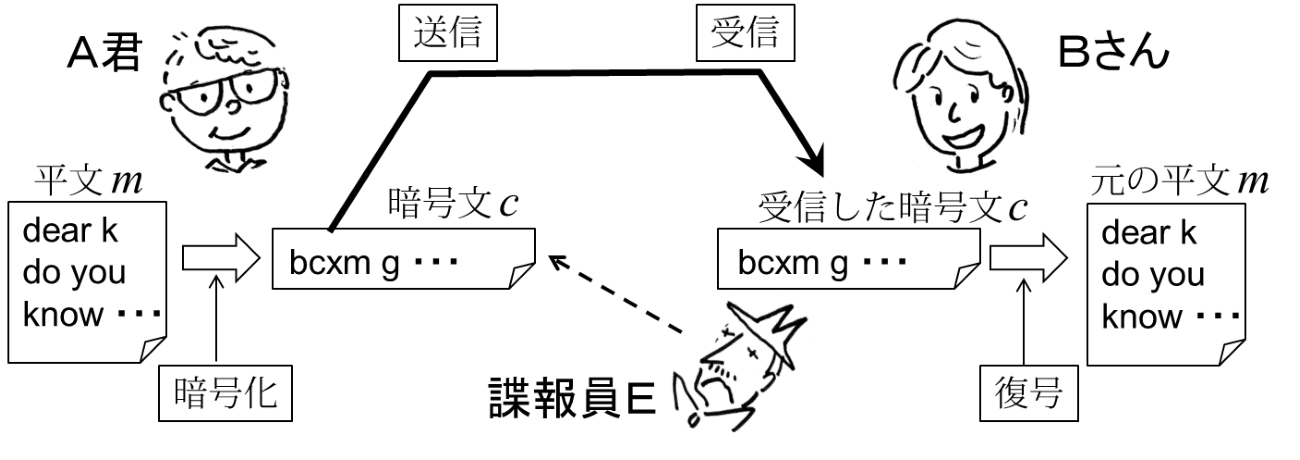
\includegraphics[scale=0.3]{./Figure/elementaryCS-figAliceBob.pdf}
  \end{center}
\end{frame}
\begin{frame}[fragile]
\frametitle{暗号方式 (Cryptography)}
  \begin{itemize}
\item シーザ暗号 (Caesar cipher): ローマ皇帝シーザが使った方式
\item ビジュネル暗号 (Vigen\`{e}re cipher): Vigen\`{e}re が作った方式
\item エニグマ (enigma): 大戦中にドイツ軍が使った方式
\item DES (Data Encyption Satandard), RSA (Rivest, Shamir and Adleman): 現在広く利用されている方式
  \end{itemize}
\end{frame}
\begin{frame}[fragile]
\frametitle{シーザ暗号}
  \begin{itemize}
\item 文字を $k$ 字先にシフトして暗号文を作る
\item \(k=3\) とすると下図のようになる
\item z, y, x は a, b, c になる
\item これからこれを関数として表していく
  \end{itemize}
  \begin{center}
    \begin{tabular}{ccccc}
a & b & c && z\\
$\downarrow$&$\downarrow$&$\downarrow$&$\cdots$&$\downarrow$\\
d & e & f && c
    \end{tabular}
  \end{center}
\end{frame}
\begin{frame}[fragile,shrink]
\frametitle{暗号システムに必要な要素}
  \begin{itemize}
\item $\cal M$: 文の集合
\item $\cal C$: 暗号文の集合
\item $\cal K$: 鍵の集合
\item \(\cal E\colon M\rightarrow C\): 暗号関数の集合
\item \(\cal D\colon C\rightarrow M\): 復号関数の集合
  \end{itemize}
  \begin{example}[Caesar Cipher]
\scriptsize
    \begin{itemize}
\item アルファベットは 0 から 25 に順番に対応付けられていると仮定する
\item $\cal M$: アルファベットの文字の列
\item $\cal C$: アルファベットの文字の列
\item $\cal K$: \(\{i\mid 0\leq i\leq 25\) であるような整数 $i\}$
\item \(\cal E\): \(\{E_k\mid k\in{\cal K}\ \mbox{and}\ \forall m(=m_1,m_2,\cdots)\in {\cal M}.E_k(m)=(m_i+k)\mod 26\}\)
\item \(\cal D\): \(\{D_k\mid k\in{\cal K}\ \mbox{and}\ \forall c(=c_1,c_2,\cdots)\in {\cal C}.D_k(k,c)=(26+c_i-k)\mod 26\}\)
    \end{itemize}
  \end{example}
\end{frame}
\begin{frame}
\frametitle{いくつかの用語}
  \begin{itemize}
\item \(E_k\in{\cal E}\) を \(m\in{\cal M}\) に適用することを暗号化 (encipher)
\item \(D_k\in{\cal D}\) を \(c\in{\cal C}\) に適用することを復号 (decipher)
\item \(k\in{\cal K}\) を 鍵 (key)
  \end{itemize}
  \begin{center}
    \begin{tabular}{ccc}
平文 (plaintext)&&暗号文 (ciphertext)\\
Hello World&$\stackrel{\mbox{暗号化}}{\rightarrow}$&Hhoor Wruog\\
Hello World&$\stackrel{\mbox{復号}}{\leftarrow}$&Hhoor Wruog
    \end{tabular}
  \end{center}
\end{frame}
\begin{frame}
\frametitle{シーザ暗号を関数であらわす}
  \begin{itemize}
\item 各文字を 0 から 25 で置き換える
    \begin{itemize}
\item a$\rightarrow$0, z$\rightarrow$25
    \end{itemize}
\item 暗号化関数 \(\mathit{enc}(3,m)=c\): 平文 \(m=m_1,m_2,\cdots,m_n\),暗号文 \(c=c_1,c_2,\cdots,c_n\) として \(f(m_i)=(m_i+3)\mod 26\) と表せる
\item 復号関数 \(\mathit{dec}(3,c)=m\): 平文 \(m=m_1,m_2,\cdots,m_n\),暗号文 \(c=c_1,c_2,\cdots,c_n\) として \(f^{-1}(c_i)=((26+c_i)-3)\mod 26\) と表せる
  \end{itemize}
  \begin{center}
    \begin{example}[Hello のシーザ暗号]
      \begin{itemize}
\item 暗号化は 関数 enc として enc(3,"Hello")="Hhoor" と表せる
\item 復号は 関数 dec として dec(3,"Hhoor")="Hello" と表せる
      \end{itemize}
    \end{example}
  \end{center}
\end{frame}
%
%%% CRYPTGRAPHY
%
\subsection{暗号通信のプログラム}
\begin{frame}[containsverbatim,shrink]
\frametitle{プログラムにしてみる}
\framesubtitle{宿題 4}
  \begin{itemize}
\item 関係として仕様をあらわしたので,実際にプログラムにしてみます
\item 具体的な計算として手続きを示した関数を定義します
\item 暗号システムという複雑なものを分割
  \end{itemize}
  \begin{lstlisting}[caption={ango.py},label=lst:ango]
# ango.py
# 暗号化サブルーチンの定義と利用
# 入力: 文字列
# 出力: 暗号化した文字列

### Global variables
K = 3 # 暗号鍵の設定

# 平文を暗号化するサブルーチン
# enc(秘密鍵 k, 平文 m) = 暗号文 c
def enc(k, m):
  ALPHABET = range(ord('a'), ord('z')+1) # 英字小文字アルファベット
  plain = list(m.encode("ascii"))        # 文字列 -> 文字コードの配列
  cipher = plain.copy()                  #暗号文格納用配列
  for i,code in enumerate(plain):
    ###
    # 宿題 4
    ###
  return(bytes(cipher).decode("ascii"))
  \end{lstlisting}
\end{frame}
\begin{frame}[containsverbatim,shrink]
\frametitle{宿題 4 (ango.py) のヒント}
  \begin{itemize}
\item \href{https://en.wikipedia.org/wiki/ASCII\#/media/File:US-ASCII\_code\_chart.png}{\beamerbutton{ASCII Code Chart}} を思い出してください
\item 小文字 a は 97 (0x61) が割り当てられています
\item アルファベットを 0 から 25 までの数字に対応づける
    \begin{itemize}
\item a の文字コード 97 を引くと文字を 0 から 25 に対応付けることができる
    \end{itemize}
\item {\tt m.encode("ascii")}で 1 バイトの文字コードの列に変換
\item {\tt list()} で配列を作成
\item 鍵 k 分だけ各整数にたす
\item 25 をこえるときは 0 にもどって計算
\item {\tt bytes(cipher).decode("ascii")}で文字の列に変換
  \end{itemize}
  \begin{center}
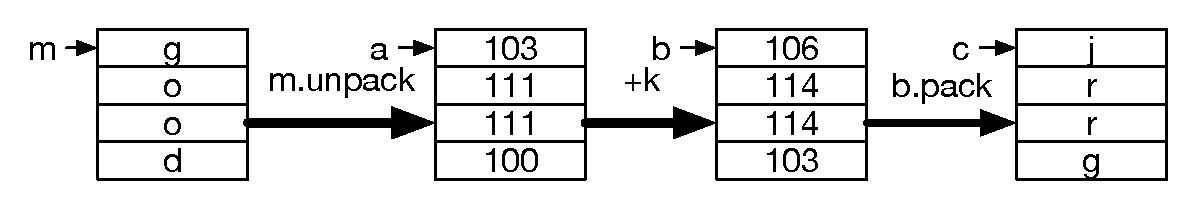
\includegraphics[scale=0.5]{./Figure/elementaryCS-figAngo.eps}
  \end{center}
\end{frame}
\begin{frame}[containsverbatim,shrink]
\frametitle{Python における文字列の操作}
  \begin{itemize}
\item {\tt str.encode("ascii")} で 1 バイトの列に変換
\item {\tt list()} で配列を作成
\item code.py を実行すると動作が見られます
  \end{itemize}
  \begin{lstlisting}[caption={code.py},label=lst:code]
# code.py
# 文字列処理の復習用
# 入力: 文字列
# 出力: 文字列の文字で小文字のみ,文字と各種情報を出力する
ALPHABET = range(ord('a'), ord('z')+1)         # 英字文字アルファベット
bun = input("Enter a string:")                 # 入力文字列から改行除法
cc  = list(bun.encode("ascii"))                # 文字列 → 文字コードの配列
for i, moji in enumerate(bun):                 # mojiはbunのi文字目を得る (i は 0 から始まる)
  code   = cc[i]                               # その文字のコードを得る
  offset = code - ALPHABET[0]                  # 文字 a との差分
  if code in ALPHABET:                         # 小文字アルファベットなら
    print(moji, ": ", code, ", ",hex(code), ", ", offset)   #   差分まで表示する
  else:                                        # そうでない時は
    print(moji, ": ", code, ", ",hex(code))    #   差分は表示しない
  \end{lstlisting}
\end{frame}
\begin{frame}[containsverbatim,shrink]
\frametitle{復号関数}
\framesubtitle{宿題 5}
  \begin{lstlisting}[caption={hukugo.py},label=lst:hukugo]
# hukugo.py
# 復号サブルーチンの定義と利用
# 入力: 暗号文の文字列
# 出力: 復号した平文
### Global variables
K = 3 # 暗号鍵の設定

# 平文を暗号化するサブルーチン
# dec(秘密鍵 k, 暗号文 c) = 平文 m
def dec(k, c):
  ALPHABET = range(ord('a'), ord('z')+1) # 英字小文字アルファベット
  cipher = list(c.encode("ascii"))       # 文字列 -> 文字コードの配列
  plain = cipher.copy()                   # 平文格納用配列
  for i,code in enumerate(cipher):
    ###
    # 宿題 5
    ###
  return(bytes(plain).decode("ascii"))
  \end{lstlisting}
\end{frame}
\begin{frame}[containsverbatim,shrink]
\frametitle{宿題 4, 5}
  \begin{itemize}
\item \href{https://sites.google.com/a/presystems.xyz/sample/home/elementary-computer-science}{\beamerbutton{https://sites.google.com/a/presystems.xyz/sample/home/elementary-computer-science}}から ango-skeleton.py と hukugo-skeleton.py をダウンロード
\item 同様にテスト用サンプルデータ plaintext.txt と ciphertext.txt をダウンロード(ソースコードと同じディレクトリに保存してください)
\item ファイル名は暗号化プログラム: ango.py, 復号プログラム: hukugo.py としてください
\item 提出は OCW-i から
  \end{itemize}
\end{frame}

%
%%% QUIZ 3
%
\part{CS 第 1\textemdash 課題 3}
\frame{
  \frametitle{CS 第 1 \textemdash 課題 3}
\scriptsize
  \tableofcontents[part=7]
}
\section{課題 3 演習ガイド}
%
%%% CRYPTANALYSIS
%
\subsection{暗号解読 (Cryptoanalysis)}
\begin{frame}[containsverbatim,shrink]
\frametitle{暗号解読}
  \begin{itemize}
\item 暗号をやぶろうとすることを暗号解読 (cryptoanalysis) と呼ぶ
\item 暗号アルゴリズム (\(\cal E\) と \(\cal D\)) は知っているが,鍵を知らないという前提
\item Cipher text only attack: 暗号文だけを得ることができるとして解読 (e.g. 踊る人形)
\item Known plaintext attack: 平文とその暗号文を得ることができるとして解読 (e.g. エニグマで "異常なし")
\item Chosen plaintext attack: 特定の平文を送り,埋め込んだ暗号文を得ることができるとして解読 (e.g. 日本軍のミッドウェイ島攻撃)
  \end{itemize}
\end{frame}
\subsection{課題 3 のシチュエーション}
\begin{frame}[containsverbatim,label=situation,shrink]
\frametitle{課題 3 のシチュエーション}
  \begin{itemize}
\item Alice と Bob が通信しているとして,そこに Eve (eavesdropper) がいるとします
\item 通信の内容を盗み見られないように暗号化して通信します
\item 暗号化の手順は以下の通り
    \begin{enumerate}
\item 送りたい文 (平文 $m$) を暗号化 (encryption) して暗号文 $c$ を作成
\item 暗号文 $c$ を送信
\item 暗号文 $c$ を受信
\item 暗号文 $c$ を復号 (decryption) して平文 $m$ を得る
    \end{enumerate}
\item Eve はこの通信の内容を盗み見て暗号文だけが入手可能で暗号解読を試みる
  \end{itemize}
  \begin{center}
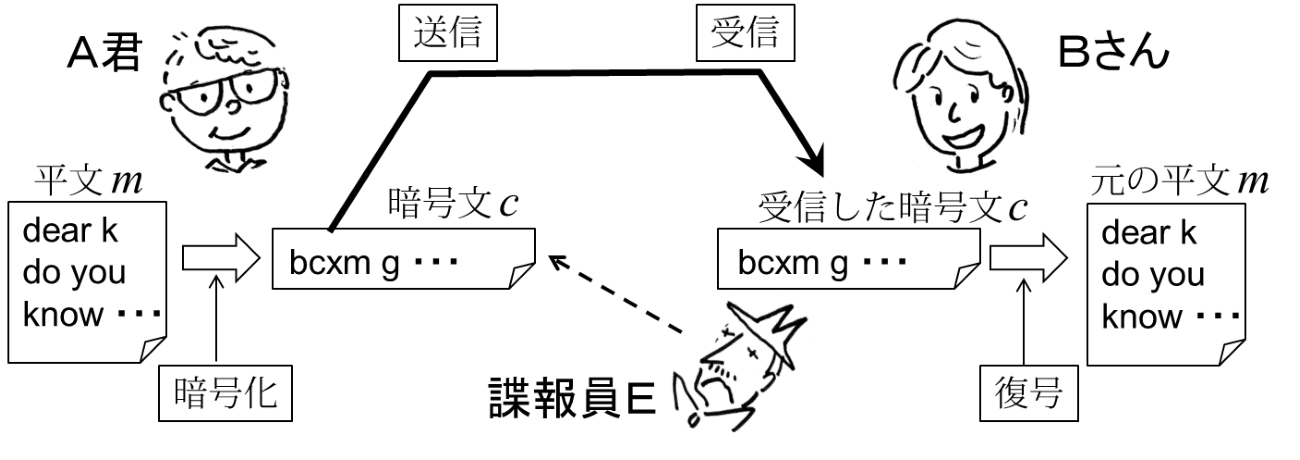
\includegraphics[scale=0.3]{./Figure/elementaryCS-figAliceBob.pdf}
  \end{center}
\end{frame}
\subsection{課題 3}
\begin{frame}[containsverbatim,shrink]
\frametitle{課題 3}
  \begin{itemize}
\item 暗号解読に挑戦
\item \href{https://sites.google.com/a/presystems.xyz/sample/home/elementary-computer-science}{\beamerbutton{https://sites.google.com/a/presystems.xyz/sample/home/elementary-computer-science}}に置いてある kaidoku-skeleton.py を参考に暗号解読プログラムを kaidoku.py を作成してください
\item 課題 3 で作成してほしいプログラム
\item 提出は OCW-i からソースコードを提出
  \end{itemize}
\end{frame}
\begin{frame}[containsverbatim,shrink]
\frametitle{暗号解読のヒント}
  \begin{itemize}
\item 意味をなす一般的な文章では文字の出現頻度には偏りがあります
\item たとえば英語では母音 e が最も出現頻度が高い
\item シーザ暗号はこの出現頻度は暗号化しても偏りは変わりません
\item この特徴を利用して何文字移動しているかを予測することができます
\item 各文字 26 個の頻度を計算するために出現回数を要素とする配列をつくる
  \end{itemize}
  \begin{center}
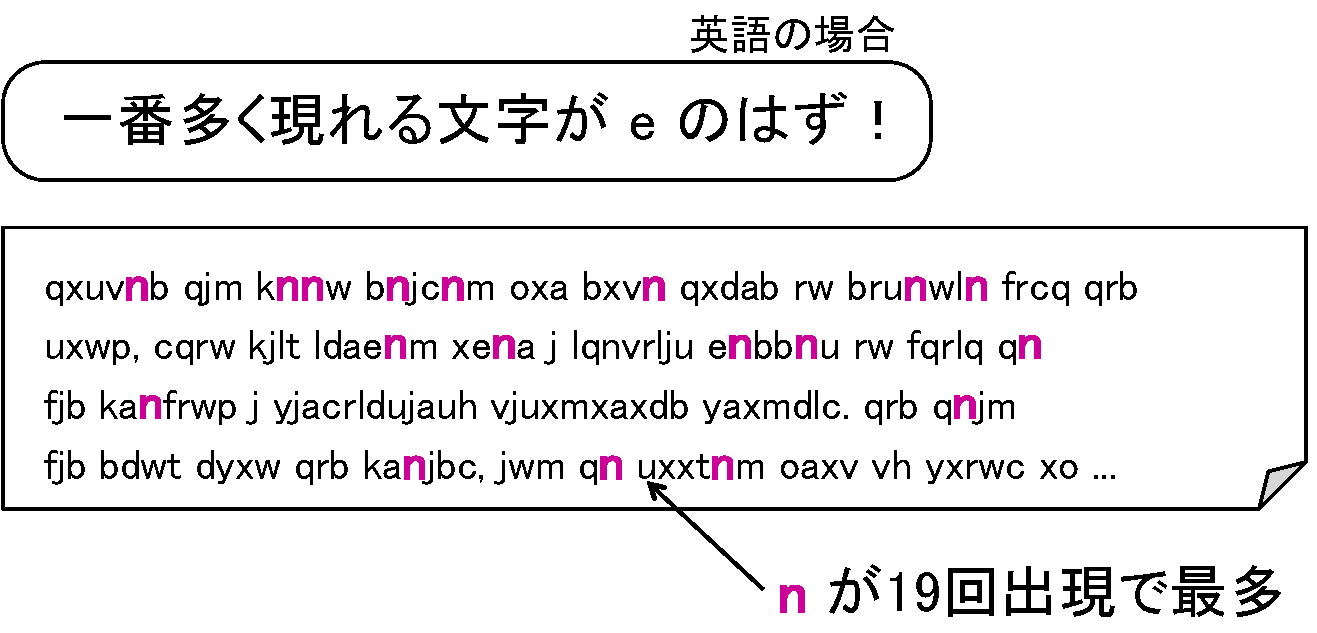
\includegraphics[scale=0.3]{./Figure/elementaryCS-figHintForCryptoanalysis.pdf}
  \end{center}
\end{frame}
\begin{frame}[containsverbatim,shrink]
\frametitle{暗号解読のヒント\textemdash つづき}
  \begin{itemize}
\item 13 番目の文字 n が最多なので 4 番目の文字 e にシフト
\item \(13-4=9\) なので 9 文字シフトしていると推測できる
  \end{itemize}
  \begin{center}
\includegraphics[scale=0.3]{./Figure/elementaryCS-figHindo.pdf}
  \end{center}
\end{frame}
\begin{frame}[containsverbatim,shrink]
\frametitle{暗号解読のヒント\textemdash より高度な方法}
  \begin{itemize}
\item フォーマルには各文字の出現頻度と暗号文での出現頻度の相関\(\phi(i)\)をとります
\item \(\phi(i)=\Sigma_{0\leq c\leq 25}f(c)p(c-i)\), ここで \(f(c)=\frac{n_c}{l_{ct}}\) は暗号文での文字 c の出現頻度,\(p(c-i)\) は一般の出現頻度とする
\item \href{https://sites.google.com/a/presystems.xyz/sample/home/elementary-computer-science}{\beamerbutton{https://sites.google.com/a/presystems.xyz/sample/home/elementary-computer-science}}に置いてある 1-gram.txt が出現頻度のファイルです
\item 相関係数 \(\phi(i)\) が
    \begin{itemize}
\item $1$ に近いほど: \(f(c)\) が大きくなれば \(p(c-i)\) も大きくなり相関が強くなる
\item $0$ 近傍: \(f(c)\) と \(p(c-i)\) はあまり相関がない
    \end{itemize}
  \end{itemize}
\end{frame}


\end{document}
